\documentclass[12pt,a4paper,oneside]{report}

% ----------------------------------------------------------
% Core packages - Overleaf compatible (pdfLaTeX)
% ----------------------------------------------------------
\usepackage[T1]{fontenc}
\usepackage[utf8]{inputenc}
\usepackage[english,french]{babel}
\usepackage{lmodern}
\usepackage{geometry}
\usepackage{setspace}
\usepackage{graphicx}
\usepackage{rotating}
\usepackage{array,booktabs,tabularx,longtable,multirow}
\usepackage{xltabular}
\usepackage{ragged2e}
\usepackage{enumitem}
\usepackage{titlesec}
\usepackage{caption}
\usepackage{subcaption}
\usepackage{fancyhdr}
\usepackage{hyperref}
\usepackage{bookmark}
\usepackage{xcolor}
\usepackage{colortbl}
\usepackage{amsmath,amssymb}
\usepackage{siunitx}
\usepackage{csquotes}
\usepackage{etoolbox}
\usepackage{ifthen}
\usepackage{listings}
\usepackage{algorithm}
\usepackage{algpseudocode}
\usepackage{tocloft}
\usepackage{emptypage}
\usepackage{pifont}
\usepackage{tcolorbox}
\usepackage{cite}
\usepackage{url}
\usepackage{xurl}
\usepackage{microtype}
\usepackage{truncate}
\usepackage{seqsplit}
\usepackage{pdfpages}
\usepackage{appendix}
\usepackage{float}
\usepackage{placeins}
\usepackage{afterpage}
\usepackage{tikz}
\usetikzlibrary{shapes.geometric, positioning, arrows.meta}

% ==========================================================
% GENERAL CONFIGURATION - ESPRIM FINAL PROJECT TEMPLATE
% Knowledge Platform final-year report
% ==========================================================

% ---------- Guide mode and final submission mode ----------
\newif\ifshowguide
\showguidefalse         % Submission version (no blue guide boxes)

% ---------- Report identity ----------
\newcommand{\AcademicYear}{2025/2026}
\newcommand{\DegreeName}{National Engineering Degree}
\newcommand{\SchoolName}{Private Higher School of Engineering of Monastir}
\newcommand{\SchoolShort}{ESPRIM}
\newcommand{\DepartmentName}{Computer Science and Information Systems}
\newcommand{\SpecialityName}{Software Engineering and Data Science}
\newcommand{\DisciplineName}{Web development}

% ---------- Title and people ----------
\newcommand{\ReportTitleFR}{Plateforme d’Intelligence de Connaissance d’Entreprise basée sur l’Intelligence
Artificielle}
\newcommand{\ReportTitleEN}{Enterprise Knowledge Intelligence Platform based on Artificial Intelligence}
\newcommand{\StudentName}{Adam Farhat}
\newcommand{\CompanyName}{HyprCraft Solutions}
\newcommand{\IndustrialSupervisor}{mohamed aziz rezgui}
\newcommand{\AcademicSupervisor}{Jacem Mhenni}
\newcommand{\JuryPresident}{Haifa Mohdhi}
\newcommand{\JuryMemberA}{Hajer Maraoui}
\newcommand{\DefenseDate}{July 24, 2026}

% ---------- Keywords ----------
\newcommand{\KeywordsFR}{RAG, recherche d'entreprise, base vectorielle, contr\^ole d'acc\`es, application web}
\newcommand{\KeywordsEN}{Retrieval-Augmented Generation, Enterprise Search, Vector Database, Access Control, Full-Stack Web Application, Large Language Models}

% ---------- Hyperref ----------
\newcommand{\PDFSubject}{Final-year project report -- Knowledge Platform}
\newcommand{\PDFKeywords}{RAG, enterprise knowledge, pgvector, Next.js, ESPRIM}

% ---------- Figures / paths ----------
\newcommand{\EsprimLogoPath}{assets/logo-esprim.png}

% ---------- Discipline hints ----------
\newcommand{\disciplinecode}{ds}

% ---------- Validation environment ----------
\newcommand{\SimilarityTarget}{< 15\%}
\newcommand{\MinReferences}{25}
\newcommand{\IndexedRatio}{\(\geq 60\%\)}


% ----------------------------------------------------------
% Page layout
% ----------------------------------------------------------
\geometry{top=2.5cm,bottom=2.5cm,left=3cm,right=2.5cm}
\setstretch{1.5}
\setlength{\parskip}{0.3em}
\setlength{\parindent}{0pt}
\emergencystretch=2em
\setlength{\headheight}{14pt}
\setcounter{secnumdepth}{3}
\setcounter{tocdepth}{2}

% ----------------------------------------------------------
% Colors and styles
% ----------------------------------------------------------
\definecolor{EsprimRed}{RGB}{166,28,33}
\definecolor{EsprimDark}{RGB}{45,45,45}
\definecolor{EsprimGrey}{RGB}{95,95,95}
\definecolor{GuideBlue}{RGB}{232,241,251}
\definecolor{GuideBorder}{RGB}{74,122,178}
\definecolor{GoodGreen}{RGB}{15,110,60}
\definecolor{WarnOrange}{RGB}{180,110,0}
\definecolor{sectionblue}{RGB}{74,122,178}

\titleformat{\chapter}[display]
  {\normalfont\bfseries\Huge\color{black}}
  {\filleft\MakeUppercase{\chaptername\ \thechapter}}
  {0.8ex}
  {\titlerule[0.8pt]\vspace{1ex}\filright}

% chaptermark stores title only; header prepends \chaptername~\thechapter (fixes ?? with titlesec [display]).
\renewcommand{\chaptermark}[1]{\markboth{#1}{#1}}

\titleformat{\section}
  {\normalfont\bfseries\Large\color{black}}
  {\thesection}{0.8em}{}

\titleformat{\subsection}
  {\normalfont\bfseries\large\color{black}}
  {\thesubsection}{0.8em}{}

\titleformat{\subsubsection}
  {\normalfont\bfseries\normalsize\color{black}}
  {\thesubsubsection}{0.8em}{}

\titleformat{\paragraph}[block]
  {\normalfont\bfseries\normalsize\color{black}}
  {}{0em}{}

\captionsetup[figure]{labelfont=bf,textfont=small,position=below,justification=justified,singlelinecheck=false}
\captionsetup[table]{labelfont=bf,textfont=small,position=above,justification=justified,singlelinecheck=false}

% List of figures/tables: short captions + room for page numbers
\setlength{\cftfigindent}{0pt}
\setlength{\cftfignumwidth}{2.8em}
\setlength{\cfttabindent}{0pt}
\setlength{\cfttabnumwidth}{2.8em}
\cftsetrmarg{2.5em plus 1fil}

% Inline-safe monospace (tables and prose). Do not use \\ inside table cells.
\newcommand{\tcode}[1]{{\footnotesize\ttfamily #1}}
\newcommand{\apicode}[1]{{\footnotesize\ttfamily\url{#1}}}
\newcommand{\tcodelines}[2]{\apicode{#1}\newline\apicode{#2}}
\newcommand{\testfile}[1]{{\footnotesize\ttfamily\seqsplit{#1}}}

% Diagram helpers (sequence + sprint-scoped use cases)
\newcommand{\seqdiagram}[4]{%
  \begin{figure}[H]
  \centering
  \includegraphics[width=0.98\textwidth,height=0.86\textheight,keepaspectratio]{assets/figures/#1.png}
  \caption[#2 --- sequence diagram]{#2 --- sequence diagram}
  \label{#4}
  \end{figure}%
}
% Structural diagrams (architecture / use-case / class) — no sequence suffix.
\newcommand{\structdiagram}[4]{%
  \begin{figure}[H]
  \centering
  \includegraphics[width=0.98\textwidth,height=0.86\textheight,keepaspectratio]{assets/figures/#1.png}
  \caption[#2]{#2}
  \label{#4}
  \end{figure}%
}
\newcommand{\sprintusecase}[3]{%
  \begin{figure}[H]
  \centering
  \includegraphics[width=\textwidth,height=0.86\textheight,keepaspectratio]{assets/figures/sprint-#1-use-case-knowledge-platform.png}
  \caption[#2]{#2}
  \label{#3}
  \end{figure}%
}
\newcommand{\sprintclass}[3]{%
  \begin{figure}[H]
  \centering
  \includegraphics[width=\textwidth,height=0.86\textheight,keepaspectratio]{assets/figures/sprint-#1-class-knowledge-platform.png}
  \caption[#2]{#2}
  \label{#3}
  \end{figure}%
}
% Sprint structural block: use-case + domain class diagrams under one subsubsection.
% #1 sprint num; #2 subsubsection title; #3/#4 usecase caption/label; #5 usecase prose;
% #6/#7 class caption/label; #8 class prose.
\newcommand{\sprintstructural}[8]{%
  \subsubsection{#2}%
  \label{subsubsec:sprint#1-structural}%
  \paragraph{Sprint~#1 use-case diagram.}%
  #5%
  \sprintusecase{#1}{#3}{#4}%
  \paragraph{Sprint~#1 domain class diagram.}%
  #8%
  \sprintclass{#1}{#6}{#7}%
}
% #1 sprint num; #2 subsubsection title (e.g. interaction sequences theme).
\newcommand{\sprintsequences}[2]{%
  \subsubsection{#2}%
  \label{subsubsec:sprint#1-sequences}%
}
\newcommand{\sprintflowgroup}[1]{%
  \par\vspace{0.6em}\noindent\textit{#1}\par\vspace{0.3em}%
}
\newcommand{\uiscreenshot}[4]{%
  \begin{figure}[H]
  \centering
  \includegraphics[width=0.92\textwidth,height=0.84\textheight,keepaspectratio]{assets/ui-screenshots/#1}
  \caption[#3]{#2}
  \label{#4}
  \end{figure}%
}
% Structured academic explanation for a UI screen (before \uiscreenshot).
\newcommand{\uiexplain}[5]{%
  \noindent\textbf{Purpose.} #1\par\vspace{0.2em}%
  \noindent\textbf{Access.} #2\par\vspace{0.2em}%
  \noindent\textbf{Main components.} #3\par\vspace{0.2em}%
  \noindent\textbf{Typical workflow.} #4\par\vspace{0.2em}%
  \noindent\textbf{Expected behaviour.} #5\par\vspace{0.35em}%
}
\newcommand{\techicon}[2][1.15em]{%
  \raisebox{-0.28\height}{\includegraphics[height=#1]{assets/tech-icons/#2.png}}%
}
\newcommand{\techiconlabel}[2]{\techicon[1.05em]{#1}\\[-0.1em]{\scriptsize #2}}

% Slightly tighter tables; consistent wrapping
% tabularx allows only ONE X column per table — use p{0.xx\linewidth} for other flexible cols
\newcolumntype{Y}{>{\RaggedRight\arraybackslash}X}
\setlength{\tabcolsep}{4pt}
\renewcommand{\arraystretch}{1.3}
\AtBeginEnvironment{tabular}{\small\setlength{\tabcolsep}{4pt}}
\AtBeginEnvironment{tabularx}{\small\setlength{\tabcolsep}{4pt}\renewcommand{\arraystretch}{1.3}}
\AtBeginEnvironment{xltabular}{\small\setlength{\tabcolsep}{4pt}\renewcommand{\arraystretch}{1.3}}
\AtBeginEnvironment{longtable}{\small\setlength{\tabcolsep}{4pt}}

\counterwithin{figure}{chapter}
\counterwithin{table}{chapter}
\counterwithin{equation}{chapter}

% ----------------------------------------------------------
% Header / footer
% ----------------------------------------------------------
\pagestyle{fancy}
\fancyhf{}
\makeatletter
\fancyhead[L]{\small\truncate{0.52\textwidth}{%
  \ifnum\value{chapter}>0 \MakeUppercase{\chaptername~\thechapter.}~\fi\nouppercase{\leftmark}%
}}
\makeatother
\fancyhead[R]{\small \SchoolShort{} -- Final Project Report}
\fancyfoot[C]{\thepage}
\renewcommand{\headrulewidth}{0.4pt}
\renewcommand{\footrulewidth}{0pt}

% ----------------------------------------------------------
% Hyperlinks
% ----------------------------------------------------------
\hypersetup{
  colorlinks=true,
  linkcolor=black,
  citecolor=black,
  urlcolor=black,
  breaklinks=true,
  pdftitle={\ReportTitleEN},
  pdfauthor={\StudentName},
  pdfsubject={\PDFSubject},
  pdfkeywords={\PDFKeywords}
}

% ----------------------------------------------------------
% Listings and pseudo-code
% ----------------------------------------------------------
\lstset{
  basicstyle=\ttfamily\small,
  breaklines=true,
  frame=single,
  numbers=left,
  numberstyle=\tiny,
  captionpos=b,
  tabsize=2,
  showstringspaces=false
}

% ----------------------------------------------------------
% Guidance boxes
% ----------------------------------------------------------
\newtcolorbox{guidebox}{
  colback=GuideBlue,
  colframe=GuideBorder,
  boxrule=0.7pt,
  arc=1.5mm,
  left=2mm,right=2mm,top=1.5mm,bottom=1.5mm,
  title=Writing and compliance guide
}

\newcommand{\guided}[1]{\ifshowguide\begin{guidebox}#1\end{guidebox}\fi}
\newcommand{\todo}[1]{\textcolor{EsprimRed}{\textbf{[To complete: #1]}}}
\newcommand{\okitem}{\textcolor{black}{\ding{51}}}
\newcommand{\warnitem}{\textcolor{black}{\ding{108}}}

% ----------------------------------------------------------
% Discipline-specific reminders
% ----------------------------------------------------------
\newcommand{\disciplinehint}{%
\ifstrequal{\disciplinecode}{ds}{
Data Science / AI-oriented project: clarify data sources, dataset quality, experimental protocol, metrics, reproducibility, bias analysis and model limitations.
}{
\ifstrequal{\disciplinecode}{eet}{
EET-oriented project: make the hardware/software architecture, interfaces, real-time constraints, safety aspects, protocols, relevant standards, measurements and test bench explicit.
}{
Mechatronics-oriented project: explain system decomposition, mechanical-electronic-control coupling, CAD aspects, kinematics/dynamics, integration strategy, performance testing and operational safety.
}}
}

% ----------------------------------------------------------
% Start document
% ----------------------------------------------------------
\begin{document}
\selectlanguage{english}

% ---------------- Front matter ----------------
\pagenumbering{roman}
\setcounter{page}{1}

% Official cover page (exact export from "Page de garde PFE")
\thispagestyle{empty}

\includepdf[pages=1,pagecommand={\thispagestyle{empty}}]{assets/cover/page-de-garde-pfe.pdf}

\cleardoublepage
\chapter*{Dedication}
\addcontentsline{toc}{chapter}{Dedication}

I dedicate this work to my parents, whose unconditional love, support, and sacrifices have been the foundation of all my achievements. Their encouragement has been a constant source of strength throughout my academic journey.

To my family and friends, I express my sincere gratitude for their continuous support, patience, and understanding during both the difficult and rewarding moments of this work.

I also dedicate this project to my own efforts and perseverance, which allowed me to overcome challenges and stay committed to my goals.

Finally, I extend my deepest appreciation to my professors, whose guidance, expertise, and dedication have greatly contributed to my learning and to the successful completion of this project.
\cleardoublepage
\chapter*{Acknowledgements}
\addcontentsline{toc}{chapter}{Acknowledgements}

I would like to express my sincere gratitude to everyone who contributed to the success of this final-year engineering project.

My thanks go first to my industrial supervisor at \CompanyName{}, for providing a meaningful problem statement, regular feedback, and access to the organisational context that shaped the requirements of the Knowledge Platform.

I am equally grateful to my academic supervisor at ESPRIM, \AcademicSupervisor{}, for methodological guidance, critical review of the technical choices, and support in aligning the deliverable with engineering-degree expectations.

I also thank the examination jury for their time and constructive evaluation, as well as the ESPRIM faculty who prepared us for this capstone experience.

Finally, I acknowledge my colleagues and peers whose discussions, testing, and code reviews improved the quality of the implemented solution.

\cleardoublepage
% ============================================================
%  abstracts.tex — Abstract (EN)
% ============================================================

\chapter*{Abstract}
\addcontentsline{toc}{chapter}{Abstract}

Organizations today generate vast volumes of internal documentation — policies,
technical guides, reports, and procedures — that remain largely inaccessible due to
fragmented storage, inadequate search tools, and the absence of structured access
governance. Employees, particularly new hires, waste significant time locating
information, asking colleagues, or making decisions without reliable knowledge backing.

This report presents the design and implementation of the \textbf{Knowledge Platform},
an enterprise-grade document management and AI-assisted question-answering system
built for teams organised by departments, with role-based access control. The platform
is developed as a TypeScript monorepo comprising a \textbf{Next.js~15} web application,
a \textbf{Node.js/Express} REST and Server-Sent Events API, \textbf{PostgreSQL with
pgvector} for hybrid retrieval, \textbf{Redis and BullMQ} for asynchronous document
ingestion, and \textbf{Google Gemini} as the sole external AI provider.

The core technical contribution is a \textbf{hybrid Retrieval-Augmented Generation
(RAG) pipeline} combining dense vector search and BM25-style full-text retrieval,
merged through weighted Reciprocal Rank Fusion (RRF), followed by LLM-based
reranking and streaming answer generation with source citations. The system enforces
department-scoped document visibility, a three-role hierarchy (Administrator, Manager,
Employee), and a feedback memory loop that uses negative user ratings to improve
future answers semantically.

Validation is grounded in \textbf{74 automated integration tests} across ten Vitest
suites, a RAG evaluation harness with automated judge metrics, and a fully reproducible
Docker Compose deployment. The project was managed using an \textbf{Agile Scrum}
methodology structured across five sprints.

\medskip
\noindent\textbf{Keywords:} \KeywordsEN
\cleardoublepage

\tableofcontents
\addcontentsline{toc}{chapter}{Table of contents}
\cleardoublepage

\listoffigures
\addcontentsline{toc}{chapter}{List of figures}
\cleardoublepage

\listoftables
\addcontentsline{toc}{chapter}{List of tables}
\cleardoublepage

\phantomsection
\addcontentsline{toc}{chapter}{List of abbreviations and acronyms}
\markboth{List of abbreviations and acronyms}{List of abbreviations and acronyms}

\noindent{\Large\bfseries List of abbreviations and acronyms\par}
\vspace{0.4\baselineskip}

\begingroup
\setlength{\parskip}{0pt}
\footnotesize
\renewcommand{\arraystretch}{1.08}
\noindent
\begin{tabular}{@{}>{\bfseries}p{2.1cm}@{\hspace{0.6em}}p{12.3cm}@{}}
\hline
Acronym & Definition \\
\hline
AI & Artificial Intelligence \\
ABAC & Attribute-Based Access Control \\
API & Application Programming Interface \\
BM25 & Best Matching 25 (lexical ranking function) \\
BullMQ & Redis-backed job queue library used for document ingest \\
CORP & Cross-Origin Resource Policy (browser security header) \\
CSP & Content Security Policy \\
CRUD & Create, Read, Update, Delete \\
CSV & Comma-Separated Values \\
DTO & Data Transfer Object \\
FR & Functional Requirement \\
HNSW & Hierarchical Navigable Small World (approximate nearest-neighbor index) \\
HTTP & Hypertext Transfer Protocol \\
HyDE & Hypothetical Document Embeddings (retrieval augmentation technique) \\
IDE & Integrated Development Environment \\
JWT & JSON Web Token \\
KPI & Key Performance Indicator \\
LLM & Large Language Model \\
MIME & Multipurpose Internet Mail Extensions (file type identification) \\
NFR & Non-Functional Requirement \\
ORM & Object-Relational Mapping (Prisma) \\
PFE & Final-Year Project (Projet de Fin d'\'Etudes) \\
RAG & Retrieval-Augmented Generation \\
RBAC & Role-Based Access Control \\
REST & Representational State Transfer \\
RRF & Reciprocal Rank Fusion \\
SSE & Server-Sent Events \\
TTL & Time To Live (cache expiration) \\
UML & Unified Modelling Language \\
\hline
\end{tabular}
\endgroup

\cleardoublepage

\ifshowguide
\input{sections/integrated_referential}
\cleardoublepage
\fi

% ---------------- Main body ----------------
\pagenumbering{arabic}
\setcounter{page}{1}

\chapter*{General introduction}
\addcontentsline{toc}{chapter}{General introduction}
\markboth{General introduction}{General introduction}

In recent years, organisations have undergone an accelerated digital transformation, leading to an exponential increase in the production of digital documents such as technical reports, internal procedures, contracts, and operational guidelines. While this information is essential for daily decision-making, it is often dispersed across multiple systems, shared drives, and communication channels, making it difficult to access efficiently.

This fragmentation of knowledge creates a significant operational challenge. Employees frequently struggle to locate relevant information, rely on informal communication channels, or recreate existing knowledge, which results in time loss, inconsistency, and reduced productivity. This issue becomes even more critical in engineering environments where accurate and timely access to information is essential.

Beyond simple document storage, organisations now require intelligent systems capable of organising knowledge, controlling access according to organisational structure, and enabling efficient retrieval of relevant information. At the same time, the increasing use of artificial intelligence introduces new opportunities for improving how users interact with internal knowledge bases, particularly through natural language interfaces.

This final-year project was conducted during an internship at \CompanyName{}. It aims to explore and address the challenges of enterprise knowledge management by designing and implementing a platform that centralizes organisational documents and improves information accessibility through intelligent search and interaction mechanisms.

The main problem addressed in this work can be stated as follows:
\emph{How can an engineering organisation structure its internal knowledge, ensure secure and role-based access to information, and enable efficient retrieval of reliable answers from its documentation?}

To address this problem, the project focuses on the following objectives:
\begin{enumerate}[leftmargin=*,itemsep=0.2em]
  \item design a secure platform supporting multiple user roles with controlled access to organisational documents;
  \item improve information retrieval from heterogeneous document sources;
  \item enable more efficient access to knowledge through intelligent assistance mechanisms;
  \item ensure system reliability through testing and validation approaches;
  \item provide a reproducible and deployable software solution.
\end{enumerate}

The scope of this project includes the design and implementation of a full-stack web application for document management and knowledge access. It covers authentication, document organisation, and intelligent retrieval functionalities, while ensuring structured access based on organisational roles and departments.

However, certain aspects remain outside the scope of this work, including mobile application development, large-scale distributed infrastructure deployment, and external enterprise authentication systems.

This report is organised as follows. Chapter~\ref{ch:state-of-the-art} presents the state of the art and positions the project within existing solutions. Chapter~\ref{ch:requirements} describes the requirements analysis and methodology. Chapter~\ref{ch:architecture} details the system design and architecture. Chapter~\ref{ch:implementation} presents the implementation process. Chapter~\ref{ch:validation} covers testing and validation. Finally, the conclusion summarises the contributions and discusses future work.
% ============================================================
%  chapter1_state_of_the_art.tex
% ============================================================
\chapter[State of the Art]{State of the Art and Project Positioning}
\label{ch:state-of-the-art}

This chapter surveys the scientific and industrial landscape relevant to enterprise
knowledge management, information retrieval, and Retrieval-Augmented Generation.
It analyses existing solutions comparatively and positions the Knowledge Platform
within this context. Implementation details, requirements, and validation are
deliberately out of scope here; they are addressed in subsequent chapters.

\section{Scientific and Technical Context}
\label{sec:context}

\subsection{The Enterprise Knowledge Lifecycle Problem}

Modern organisations face a fundamental challenge in managing knowledge at scale. On one hand, they continuously generate large volumes of heterogeneous digital assets, including technical documentation, procedures, contracts, internal reports, spreadsheets, emails, and operational guidelines. On the other hand, these assets are distributed across multiple disconnected systems such as shared drives, email platforms, messaging tools, and departmental repositories.

This fragmentation creates a structural inefficiency that goes beyond retrieval. Enterprise knowledge is difficult not only to find, but also to:

\begin{itemize}
    \item collect in a structured and consistent manner;
    \item centralize across heterogeneous tools and departments;
    \item organize according to business logic and ownership;
    \item govern through access control policies;
    \item retrieve in a meaningful and context-aware way.
\end{itemize}

As a result, employees often rely on informal communication or personal experience instead of documented knowledge. Studies show that knowledge workers spend a significant portion of their time searching for information rather than performing productive tasks \cite{gao2024rag-survey}.

\subsection{Limitations of Traditional Document Systems}

Traditional enterprise tools such as Google Drive, OneDrive, and Microsoft SharePoint were primarily designed for storage and collaboration rather than intelligent knowledge management.

While they provide reliable file storage and basic access control, they suffer from key limitations:

\begin{itemize}
    \item lack of semantic understanding of content;
    \item keyword-based search that ignores meaning and context;
    \item weak knowledge structuring and duplication of information;
    \item limited ability to answer questions directly;
    \item coarse-grained permission models not aligned with organizational logic.
\end{itemize}

These systems function as passive repositories rather than active knowledge systems.

\section{Information Retrieval: From Keywords to Semantics}

\subsection{Classical Retrieval Models}

Traditional information retrieval relies on lexical matching approaches such as TF-IDF and BM25 \cite{robertson2009bm25}. These methods rank documents based on term frequency and inverse document frequency, making them effective for exact keyword matching.

However, they fail to capture semantic similarity. Two expressions with identical meaning but different wording may not match, which limits their effectiveness in enterprise contexts.

\subsection{Dense Retrieval and Semantic Search}

Dense retrieval methods address this limitation by encoding queries and documents into continuous vector representations \cite{karpukhin2020dpr, reimers2019sentence}. This enables semantic matching between conceptually similar texts even when lexical overlap is low.

Despite their advantages, dense retrieval models also have limitations:

\begin{itemize}
    \item weaker performance on rare or technical terms;
    \item sensitivity to embedding model quality;
    \item reduced interpretability of ranking decisions.
\end{itemize}

\subsection{Hybrid Retrieval Systems}

To overcome these limitations, modern systems adopt hybrid retrieval strategies that combine lexical and semantic approaches \cite{ram2023hybrid, lin2021unicoil}. Results are typically merged using ranking fusion techniques such as Reciprocal Rank Fusion (RRF), which balances precision and recall.

This hybrid approach is now widely considered the standard for enterprise search systems.

\section{Retrieval-Augmented Generation (RAG)}

\subsection{Concept and Architecture}

Retrieval-Augmented Generation (RAG) \cite{lewis2020rag} enhances traditional retrieval systems by integrating Large Language Models (LLMs). Instead of returning documents, the system retrieves relevant passages and uses them as context for answer generation.

A typical RAG pipeline consists of:
\begin{enumerate}
    \item a retriever that selects relevant document chunks;
    \item an optional reranker that refines retrieval quality;
    \item a generator that produces a grounded natural language response.
\end{enumerate}

\subsection{Advantages of RAG}

RAG systems provide several advantages over standalone LLMs:

\begin{itemize}
    \item factual grounding in external documents;
    \item reduced hallucination through retrieval constraints;
    \item ability to update knowledge without retraining models;
    \item improved traceability through source citations.
\end{itemize}

\subsection{Limitations in Enterprise Context}

Despite their advantages, RAG systems introduce new challenges:

\begin{itemize}
    \item strong dependency on retrieval quality;
    \item sensitivity to chunking and indexing strategies;
    \item difficulty in systematic evaluation;
    \item lack of native access control mechanisms;
    \item complexity of production deployment.
\end{itemize}

\subsection{Evaluation of RAG Systems}

Evaluating RAG systems remains a complex task, as classical IR metrics do not capture answer quality or factual grounding. Recent research proposes LLM-based evaluation frameworks that assess faithfulness, relevance, and completeness of generated answers \cite{es2024rag-eval}. These methods enable automated detection of hallucinations and quality regressions in production systems.

\section{Access Control and Knowledge Governance}

\subsection{Role-Based Access Control (RBAC)}

Role-Based Access Control (RBAC) \cite{sandhu1996rbac, ferraiolo2001rbac} is the standard model for managing permissions in enterprise systems. Users are assigned to roles, and roles are associated with permissions over resources.

This model simplifies administration and supports organizational scalability.

\subsection{Challenges in Knowledge Systems}

In knowledge platforms, access control must be enforced beyond simple document visibility. It must govern:

\begin{itemize}
    \item which documents can be retrieved during search;
    \item which sources can influence generated answers;
    \item cross-department boundaries and hierarchical structures;
    \item auditability of access and usage history.
\end{itemize}

A critical requirement is that access control must be applied at the retrieval layer to prevent information leakage in generated responses.

\section{Enterprise Knowledge Systems and Existing Solutions}

\subsection{Shared Drives and Document Management Systems}

Systems such as Google Drive, OneDrive, and Microsoft SharePoint \cite{microsoft-sharepoint} provide foundational document storage and collaboration capabilities.

\textbf{Strengths:}
\begin{itemize}
    \item reliable storage and synchronization;
    \item basic access control mechanisms;
    \item widespread enterprise adoption.
\end{itemize}

\textbf{Limitations:}
\begin{itemize}
    \item lack of semantic search;
    \item no question-answering capabilities;
    \item weak knowledge structuring;
    \item folder-based organization not aligned with knowledge flows.
\end{itemize}

\subsection{Vector Databases and RAG Frameworks}

Tools such as Pinecone, Weaviate, LangChain, and LlamaIndex \cite{pinecone-docs, langchain-docs, llamaindex-docs} provide infrastructure for building retrieval systems.

\textbf{Strengths:}
\begin{itemize}
    \item scalable semantic retrieval;
    \item modular RAG pipeline construction;
    \item flexible architecture for developers.
\end{itemize}

\textbf{Limitations:}
\begin{itemize}
    \item no complete end-user system;
    \item no document lifecycle management;
    \item no access control or governance layer;
    \item significant engineering effort required for production use.
\end{itemize}

\subsection{Commercial AI Copilots}

Solutions such as Microsoft Copilot and ChatGPT Enterprise \cite{microsoft-copilot} provide conversational interfaces over enterprise data.

\textbf{Strengths:}
\begin{itemize}
    \item natural language interaction;
    \item strong ecosystem integration;
    \item low adoption barrier.
\end{itemize}

\textbf{Limitations:}
\begin{itemize}
    \item limited transparency in retrieval mechanisms;
    \item restricted control over embedding and ranking strategies;
    \item vendor lock-in;
    \item limited customization of access control logic.
\end{itemize}

\subsection{Knowledge Base Platforms}

Tools such as Guru and Tettra focus on structured knowledge management.

\textbf{Strengths:}
\begin{itemize}
    \item organized documentation workflows;
    \item curated and validated content;
    \item team-oriented knowledge sharing.
\end{itemize}

\textbf{Limitations:}
\begin{itemize}
    \item manual content creation required;
    \item no automated ingestion pipelines;
    \item limited or no AI-based retrieval;
    \item not suitable for large unstructured corpora.
\end{itemize}

\subsection{Enterprise AI Search Systems (Glean)}

Enterprise solutions such as Glean represent the most advanced commercial attempt at unified knowledge search.

\textbf{Strengths:}
\begin{itemize}
    \item unified search across multiple enterprise data sources;
    \item natural language question answering with citations;
    \item strong user experience and integration capabilities.
\end{itemize}

\textbf{Limitations:}
\begin{itemize}
    \item proprietary and closed architecture;
    \item no transparency in retrieval pipeline;
    \item no self-hosting or full customization;
    \item limited support for feedback-driven optimization.
\end{itemize}

\section{Comparative Analysis}

\begin{table}[htbp]
\centering
\caption{Comparative analysis of enterprise knowledge management solutions}
\label{tab:state-of-art}
\small
\renewcommand{\arraystretch}{1.3}
\begin{tabularx}{\textwidth}{|>{\RaggedRight\arraybackslash}p{2.3cm}|>{\RaggedRight\arraybackslash}p{0.27\linewidth}|>{\RaggedRight\arraybackslash}p{0.27\linewidth}|Y|}
\hline
\textbf{Solution} & \textbf{Strengths} & \textbf{Limitations} & \textbf{Relevance to this work} \\
\hline
Shared Drives (Drive, SharePoint) &
Reliable storage and basic access control &
No semantic search, no QA, weak structuring &
Baseline storage layer only \\
\hline
Vector DB + RAG frameworks &
Strong retrieval and modular pipelines &
No full system or governance layer &
Core retrieval component only \\
\hline
Commercial Copilots &
Ease of use and enterprise integration &
Black-box systems, limited control &
Demonstrates demand but lacks transparency \\
\hline
Knowledge Base Tools &
Structured documentation workflows &
Manual maintenance, no scalable ingestion &
Not suitable for large corpora \\
\hline
Glean &
Unified enterprise AI search with citations &
Closed system, no customization or transparency &
Closest industrial solution but not open \\
\hline
\textbf{Proposed System} &
Hybrid RAG + RBAC + full lifecycle + feedback loop &
External LLM dependency &
Full enterprise knowledge lifecycle solution \\
\hline
\end{tabularx}
\end{table}

\section{Project Positioning}

The analysis reveals a structural gap in existing solutions: no system simultaneously addresses document lifecycle management, centralized governance, semantic retrieval, and controlled AI-based question answering in a unified and transparent architecture.

The \textbf{Knowledge Platform} addresses this gap through:

\begin{itemize}
    \item centralized document ingestion and organization;
    \item role-based and department-scoped access control;
    \item hybrid lexical and semantic retrieval;
    \item Retrieval-Augmented Generation with source grounding;
    \item feedback-driven improvement mechanisms;
    \item full production-grade system architecture.
\end{itemize}

Unlike existing tools that focus on isolated components, this work proposes a complete and integrated enterprise knowledge lifecycle system.

\subsection{Key Contribution}

This work contributes a unified approach that ensures:

\begin{itemize}
    \item knowledge is properly collected and centralized;
    \item access is securely governed and auditable;
    \item retrieval is hybrid and semantically aware;
    \item answers are grounded and traceable;
    \item the system is fully reproducible and production-ready.
\end{itemize}

\section{Chapter Conclusion}

The state-of-the-art analysis highlighted the limits of traditional document
platforms and motivated a hybrid retrieval and RAG-based approach adapted to
enterprise governance constraints. By comparing existing solutions and defining
the project positioning, this chapter justified the need for an integrated
knowledge platform combining lifecycle management, controlled access, semantic
search, and grounded AI assistance. Chapter~\ref{ch:requirements} translates
these insights into functional and non-functional requirements and defines the
Agile Scrum methodology adopted for delivery.
% ============================================================
%  chapter2_requirements_methodology.tex
% ============================================================
\chapter[Requirements and Methodology]{Requirements Analysis, Specifications and Methodology}
\label{ch:requirements}

This chapter translates the gaps identified in Chapter~\ref{ch:state-of-the-art} into
a verifiable specification for the Knowledge Platform. It analyses the host-organisation
context, defines functional and non-functional requirements with acceptance criteria,
and establishes the Agile Scrum methodology and five-sprint delivery plan that
structure the design (Chapter~\ref{ch:architecture}), implementation
(Chapter~\ref{ch:implementation}), and validation (Chapter~\ref{ch:validation})
chapters.

\section{Analysis of the Existing Situation and Usage Context}

\subsection{Host Organisation Context}

\textbf{\CompanyName} is a technology company whose teams produce and consume
significant volumes of internal documentation: technical specifications, onboarding
guides, project reports, API references, and operational procedures. Prior to this
project, knowledge was distributed across disconnected tools — shared drives, email
threads, and informal messaging channels — with no unified governance model and no
mechanism for intelligent retrieval.

The key pain points identified through analysis of the existing situation were:

\begin{itemize}
  \item \textbf{Fragmented storage}: documents resided in multiple systems with no
    single point of access, making comprehensive search impossible.
  \item \textbf{No access governance}: there was no systematic control over which
    teams or roles could access which documents, leading to either over-sharing or
    information silos.
  \item \textbf{Keyword-only search}: retrieval was limited to filename and keyword
    matching, returning documents rather than answers.
  \item \textbf{Onboarding friction}: new employees had no reliable way to find answers
    to operational questions, creating repeated interruptions to experienced colleagues.
  \item \textbf{No feedback mechanism}: when information found through search was
    incorrect or outdated, there was no way to signal this or prevent the same error
    from recurring.
\end{itemize}

\subsection{System Actors}

Four actor groups interact with the Knowledge Platform, as summarized in
Table~\ref{tab:actors} and detailed in the global use-case diagram
(Subsection~\ref{subsec:global-use-case}, Figure~\ref{fig:use-cases}):

\begin{table}[H]
\centering
\caption{System actors and their primary capabilities}
\label{tab:actors}
\renewcommand{\arraystretch}{1.4}
\begin{tabularx}{\textwidth}{|>{\RaggedRight\arraybackslash}p{2.8cm}|Y|}
\hline
\rowcolor{sectionblue!15}
\textbf{Actor} & \textbf{Primary capabilities} \\
\hline
\textbf{Employee} &
Browse and search the document library, perform semantic search and RAG
question-answering, manage personal profile, maintain conversation history,
and rate assistant answers. \\
\hline
\textbf{Manager} &
All Employee capabilities, plus access to the manager dashboard showing
managed departments and their members, and the ability to send announcements
to managed departments. \\
\hline
\textbf{Administrator} &
Full platform control: user lifecycle management, department CRUD and merge,
per-user restrictions, bulk operations, audit log access, KPI dashboards,
activity exports, and platform-wide notifications. \\
\hline
\textbf{System} &
Autonomous actor: executes the BullMQ ingest worker (extract, chunk, embed),
emits automatic notifications on document and role events, and runs the RAG
evaluation harness. \\
\hline
\end{tabularx}
\end{table}

\subsection{Global Use-Case Model}
\label{subsec:global-use-case}

Figure~\ref{fig:use-cases} presents the global use-case model of the Knowledge
Platform. It identifies primary actors (\textbf{Guest}, \textbf{Employee},
\textbf{Manager}, and \textbf{Administrator}), with the three authenticated roles
generalizing an abstract \textbf{Authenticated user} actor. Use cases are grouped
into authentication, document management, search and AI, notifications, and
governance domains. Secondary actors (\textbf{Email}, \textbf{Gemini}, and
\textbf{BullMQ worker}) model external interactions through
\texttt{<<notify>>}, \texttt{<<invoke>>}, and \texttt{<<enqueue>>} dependencies.

\begin{figure}[H]
  \centering
  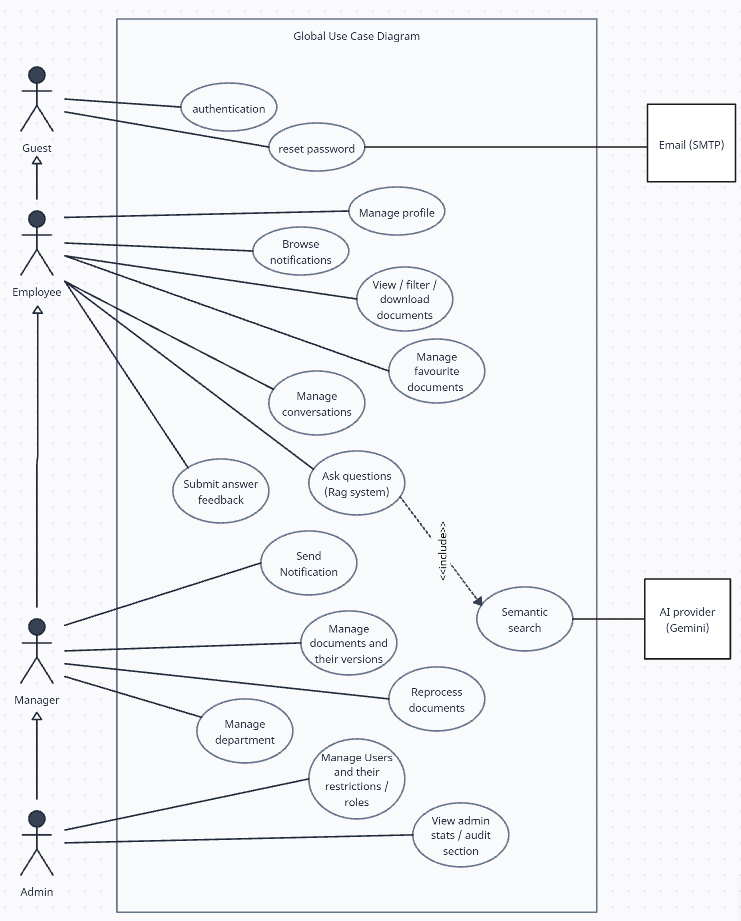
\includegraphics[width=\textwidth]{assets/figures/global-use-case-knowledge-platform.png}
  \caption{Global use-case diagram of the Knowledge Platform}
  \label{fig:use-cases}
\end{figure}

The use-case packages map directly to the functional requirement domains in
Table~\ref{tab:requirements}: authentication (FR-01, FR-02, FR-12), document
management (FR-03 to FR-05), search and AI (FR-06 to FR-08), notifications
(FR-09), and governance (FR-10, FR-11).

\section{Functional and Non-Functional Requirements}

The requirements were derived from an analysis of user workflows and system
architecture, ensuring alignment between functional needs and system design.

\subsection{Functional Requirements}

The system defines a set of functional requirements organized around
\textbf{authentication} (FR-01, FR-02), \textbf{document management} (FR-03 to
FR-05), \textbf{search and AI capabilities} (FR-06 to FR-08),
\textbf{notifications} (FR-09), \textbf{administration} (FR-10, FR-11), and
\textbf{system-level feature controls} (FR-12). Access to all functionalities is
governed by a hybrid authorization model combining Role-Based Access Control
(RBAC), Attribute-Based Access Control (ABAC), and per-user restriction flags
(see Subsection~\ref{subsec:access-control-model}).

\begin{xltabular}{\linewidth}{|>{\RaggedRight\arraybackslash}p{0.85cm}|>{\RaggedRight\arraybackslash}p{0.24\linewidth}|>{\RaggedRight\arraybackslash}p{0.31\linewidth}|Y|}
\caption{Functional requirements with acceptance criteria}
\label{tab:requirements} \\
\hline
\rowcolor{sectionblue!15}
\textbf{ID} & \textbf{Requirement} & \textbf{Acceptance criterion} & \textbf{Module / API} \\
\hline
\endfirsthead
\hline
\rowcolor{sectionblue!15}
\textbf{ID} & \textbf{Requirement} & \textbf{Acceptance criterion} & \textbf{Module / API} \\
\hline
\endhead
\hline
\endfoot

FR-01 &
JWT authentication with HttpOnly refresh cookie rotation &
Login returns access token; refresh rotates session atomically; replay revokes family &
\tcodelines{POST /auth/login}{POST /auth/refresh} \\
\hline
FR-02 &
User profile management including avatar upload &
Platform-hosted avatar served with correct CORP header; cross-origin display verified &
\tcodelines{PATCH /auth/profile}{GET /avatars/:id} \\
\hline
FR-03 &
Document upload with multi-format extraction and async ingest &
File stored on disk; ingest job enqueued; version status reaches READY &
\apicode{POST /documents/upload}\newline BullMQ worker \\
\hline
FR-04 &
Document visibility control (ALL / DEPARTMENT / PRIVATE) &
Unauthorised access returns 404 (not 403) to prevent enumeration &
\tcode{canReadDocument}\newline\tcode{documentAccess.ts} \\
\hline
FR-05 &
Document metadata: tags, favorites, recents, archive &
Tag autocomplete, favorite toggle, recent view, archive/restore all persisted &
\tcode{documents.ts} \\
\hline
FR-06 &
Semantic vector search over department-scoped document corpus &
Vector similarity results ranked correctly; access-filtered; respects restrictions &
\apicode{POST /search/semantic} \\
\hline
FR-07 &
Hybrid RAG Ask with SSE streaming and source citations &
SSE events emitted in order: \tcode{sources}, \tcode{token}, \tcode{done}; citations reference real chunks &
\tcodelines{POST /search/ask}{ragCompletion.ts} \\
\hline
FR-08 &
Conversation history with per-message feedback &
Threads persisted; thumbs up/down stored; feedback stats available to admin &
\apicode{/conversations/*} \\
\hline
FR-09 &
Automatic and manual notification system with attachments &
Department-scoped events emitted on document create/update/delete; manual send available to managers/admins &
\tcodelines{/notifications/*}{notificationService.ts} \\
\hline
FR-10 &
Full administrative control: user/department CRUD, bulk operations, audit &
Last-admin safety enforced; CSV imports escaped; audit log exportable &
\apicode{/admin/*} \\
\hline
FR-11 &
Manager dashboard scoped to manageable departments &
Only departments from \tcode{manageable\-DepartmentIds} returned; member list correct &
\apicode{/manager/*} \\
\hline
FR-12 &
Per-user feature restriction flags &
Flags block login, document access, and AI queries via middleware; restricted page displayed &
\tcode{requireDoc\-LibraryAccess}\newline\tcode{requireUse\-AiQueries} \\
\hline
\end{xltabular}

Table~\ref{tab:fr-traceability} summarises the mapping from each functional
requirement to its primary implementation module and development sprint.

\begin{table}[H]
\centering
\caption{Functional requirements traceability summary}
\label{tab:fr-traceability}
\renewcommand{\arraystretch}{1.35}
\begin{tabularx}{\textwidth}{|>{\RaggedRight\arraybackslash}p{0.85cm}|>{\RaggedRight\arraybackslash}p{2.6cm}|Y|>{\Centering\arraybackslash}p{1.0cm}|}
\hline
\rowcolor{sectionblue!15}
\textbf{ID} & \textbf{Domain} & \textbf{Primary module / service} & \textbf{Sprint} \\
\hline
FR-01 & Authentication & \tcode{auth.ts} (JWT, refresh families) & S1 \\
\hline
FR-02 & Profile management & \tcode{auth.ts}, \tcode{avatarsPublic.ts} & S1 \\
\hline
FR-03 & Document ingest & BullMQ ingest worker, \tcode{documents.ts} & S2 \\
\hline
FR-04 & Access control & \tcode{documentAccess.ts}, visibility filters & S2 \\
\hline
FR-05 & Document organisation & \tcode{documents.ts} (tags, favorites, archive) & S2 \\
\hline
FR-06 & Semantic search & \tcode{search.ts}, pgvector retrieval & S3 \\
\hline
FR-07 & RAG question answering & \tcode{ragCompletion.ts} (hybrid RAG pipeline) & S3 \\
\hline
FR-08 & Conversations & \tcode{conversations.ts} & S3 \\
\hline
FR-09 & Notifications & \tcode{notificationService.ts}, \tcode{notifications.ts} & S4 \\
\hline
FR-10 & Administration & \tcode{admin.ts} & S4 \\
\hline
FR-11 & Manager dashboard & \tcode{manager.ts} & S4 \\
\hline
FR-12 & Feature restrictions & Auth middleware, \tcode{requireUseAiQueries} & S1 \\
\hline
\end{tabularx}
\end{table}

Chapter~\ref{ch:architecture} extends this summary with design elements and
validation test references (Table~\ref{tab:traceability-main}).

\subsection{Non-Functional Requirements}

\begin{table}[H]
\centering
\caption{Non-functional requirements}
\label{tab:nfr}
\renewcommand{\arraystretch}{1.4}
\begin{tabularx}{\textwidth}{|>{\RaggedRight\arraybackslash}p{0.85cm}|>{\RaggedRight\arraybackslash}p{0.38\linewidth}|Y|}
\hline
\rowcolor{sectionblue!15}
\textbf{ID} & \textbf{Requirement} & \textbf{Acceptance criterion} \\
\hline
NFR-01 & Health monitoring endpoint &
\tcode{GET /health} returns \tcode{200 \{status: "ok"\}} when PostgreSQL and Redis
are reachable; \tcode{503} with per-check detail otherwise \\
\hline
NFR-02 & Security headers and rate limiting &
Helmet CSP enforced on all responses; login limited to 15 req/15 min/IP; Ask
limited to 12 req/min/IP \\
\hline
NFR-03 & Single-flight refresh token (web client) &
Parallel requests from the same tab do not trigger multiple \tcode{/auth/refresh}
calls; the in-flight promise is shared \\
\hline
NFR-04 & Docker Compose reproducibility &
\tcode{docker compose up -{}-build} starts all four services (postgres, redis, api,
web) in a healthy state; migrations run automatically \\
\hline
NFR-05 & Integration test coverage &
All Vitest/Supertest suites pass on a real PostgreSQL + Redis instance with seeded
data \\
\hline
NFR-06 & RAG evaluation harness &
\tcode{npm run eval:rag:quick} executes without error and writes a JSON report
to \tcode{eval-reports/} \\
\hline
\end{tabularx}
\end{table}

\subsection{Access Control Model}
\label{subsec:access-control-model}

Building on the RBAC concepts introduced in Chapter~\ref{ch:state-of-the-art},
the platform enforces a \textbf{hybrid authorization model} that operates at three
complementary layers. This subsection specifies how the theoretical foundations are
applied to the requirements defined above.

\begin{itemize}
  \item \textbf{Role-Based Access Control (RBAC)}: every user holds one platform
    role --- \texttt{ADMIN}, \texttt{MANAGER}, or \texttt{EMPLOYEE} --- that
    determines coarse-grained capabilities. Administrators manage users,
    departments, and platform configuration (FR-10); managers access
    department-scoped dashboards and announcements (FR-11); employees use the
    document library, search, and AI assistant within their permitted scope.
  \item \textbf{Attribute-Based Access Control (ABAC)}: permissions are further
    constrained by attributes such as department membership and document
    visibility (\texttt{ALL}, \texttt{DEPARTMENT}, \texttt{PRIVATE}). Retrieval
    and RAG pipelines apply these filters before returning results, ensuring that
    semantic search and generated answers never expose unauthorised content
    (FR-04, FR-06, FR-07).
  \item \textbf{Per-user feature restriction flags}: administrators can disable
    specific capabilities for individual users --- for example, blocking document
    library access or AI queries --- via middleware that intercepts requests
    before business logic executes (FR-12).
\end{itemize}

This layered model ensures fine-grained control over system capabilities while
maintaining scalability and security across authentication, document management,
search, and AI workflows.

\section{Specifications and Performance Indicators}

The following Key Performance Indicators (KPIs) link requirements to the validation
chapter (Chapter~\ref{ch:validation}):

\begin{table}[H]
\centering
\caption{Key performance indicators}
\label{tab:kpis}
\renewcommand{\arraystretch}{1.4}
\begin{tabularx}{\textwidth}{|>{\RaggedRight\arraybackslash}p{2.5cm}|Y|>{\RaggedRight\arraybackslash}p{2.0cm}|}
\hline
\rowcolor{sectionblue!15}
\textbf{KPI} & \textbf{Measurement method} & \textbf{Target} \\
\hline
Ingest reliability &
Percentage of uploaded documents reaching \tcode{READY} status without
\tcode{FAILED} &
$\geq 95\%$ \\
\hline
Integration test pass rate &
\tcode{npm run test:api} output: passed / total &
74 / 74 (100\%) \\
\hline
RAG topic classification (no API key) &
\tcode{eval:rag:quick} optimizer pass rate &
$\geq 15/34$ (degraded mode) \\
\hline
RAG judge scores (with API key) &
Faithfulness and relevance from automated judge &
Documented in eval report \\
\hline
Security: refresh replay &
Reuse of rotated token triggers family revocation &
Verified by auth test suite \\
\hline
Security: avatar CORP &
\tcode{Cross-Origin-Resource-Policy: cross-origin} header present on avatar responses &
Verified by avatars test \\
\hline
\end{tabularx}
\end{table}

\section{Selected Methodology}

\subsection{Agile Scrum Framework}

The project was managed using the \textbf{Agile Scrum} methodology, chosen for its
iterative structure, its emphasis on working deliverables at the end of each sprint,
and its adaptability to evolving requirements — all well-suited to a complex full-stack
product developed by a single engineer over a bounded internship period.

\subsubsection{Scrum Roles}

\begin{itemize}
  \item \textbf{Product Owner}: \IndustrialSupervisor{} (\CompanyName), responsible
    for validating feature priorities and acceptance criteria.
  \item \textbf{Scrum Master / Developer}: \StudentName, responsible for sprint
    planning, execution, daily self-review, and retrospective.
  \item \textbf{Academic Advisor}: \AcademicSupervisor{} (ESPRIM), providing
    methodological and scientific guidance at sprint boundaries.
\end{itemize}

\subsubsection{Scrum Artefacts}

\begin{itemize}
  \item \textbf{Product Backlog}: the complete list of functional and non-functional
    requirements (FR-01 to FR-12, NFR-01 to NFR-06) prioritised by business value
    and technical dependency.
  \item \textbf{Sprint Backlog}: the subset of backlog items committed to in each
    sprint, decomposed into implementation tasks.
  \item \textbf{Increment}: a working, tested vertical slice of the platform delivered
    at the end of each sprint.
  \item \textbf{Definition of Done}: a requirement is considered done when (a) the
    feature is implemented, (b) at least one integration test covers the happy path
    and one error path, and (c) the corresponding API route or module is manually
    validated.
\end{itemize}

\subsubsection{Sprint Structure}

Each sprint followed a fixed rhythm:

\begin{enumerate}
  \item \textbf{Sprint Planning}: review backlog, select items, decompose into tasks,
    estimate effort.
  \item \textbf{Development}: implement features, write integration tests, perform
    code review against security and style guidelines.
  \item \textbf{Sprint Review}: demonstrate the working increment; validate against
    acceptance criteria.
  \item \textbf{Sprint Retrospective}: identify what worked, what blocked, and what
    to improve in the next sprint.
\end{enumerate}

\subsection{Sprint Plan}

The project was structured across \textbf{five sprints}, each delivering a coherent
and independently testable platform capability. Detailed interaction design for each
sprint appears in Section~\ref{sec:sprint-design} of Chapter~\ref{ch:architecture}.

\begin{table}[H]
\centering
\caption{Agile Scrum sprint plan}
\label{tab:sprints}
\footnotesize
\renewcommand{\arraystretch}{1.3}
\setlength{\tabcolsep}{2.5pt}
\begin{tabularx}{\linewidth}{|>{\Centering\arraybackslash}p{0.055\linewidth}|>{\RaggedRight\arraybackslash}p{0.16\linewidth}|>{\RaggedRight\arraybackslash}X|>{\RaggedRight\arraybackslash}p{0.13\linewidth}|>{\Centering\arraybackslash}p{0.055\linewidth}|}
\hline
\rowcolor{sectionblue!15}
\textbf{Spr.} & \textbf{Theme} & \textbf{Deliverables} & \textbf{Req.} & \textbf{Des.} \\
\hline
\textbf{S1} &
Auth., users, RBAC &
JWT login/logout/refresh (HttpOnly cookies), refresh-token family revocation,
password policy, session cap, per-user restrictions, profile/avatar, RBAC middleware &
FR-01, FR-02, FR-12 \newline NFR-02, NFR-03 &
\ref{subsec:sprint1-design} \\
\hline
\textbf{S2} &
Document library \& ingest &
Multi-format upload (PDF, Office, HTML, XML, ZIP), BullMQ worker
(extract$\to$chunk$\to$embed$\to$persist), versioning, tags, favorites, recents,
archive, visibility, audit log &
FR-03, FR-04, FR-05 &
\ref{subsec:sprint2-design} \\
\hline
\textbf{S3} &
Hybrid RAG \& Ask &
Query optimiser, hybrid retrieval (pgvector + BM25 + RRF), LLM reranking,
neighbour expansion, SSE answers with citations, confidence scoring, critique,
claim verification, follow-ups, feedback loop, conversations &
FR-06, FR-07, FR-08 \newline NFR-06 &
\ref{subsec:sprint3-design} \\
\hline
\textbf{S4} &
Admin, manager, notifications &
Admin CRUD (users, departments, merge, bulk ops, CSV), dept-access management,
KPI dashboard, activity/audit exports, manager view, auto/manual notifications &
FR-09, FR-10, FR-11 &
\ref{subsec:sprint4-design} \\
\hline
\textbf{S5} &
Tests, eval \& deploy &
74 Vitest/Supertest integration tests, RAG eval CLI (automated judge),
Docker Compose prod config, migration pipeline, 54 UML diagrams, README &
NFR-01, NFR-04, NFR-05 \newline NFR-06 &
\ref{subsec:sprint5-design} \\
\hline
\end{tabularx}
\end{table}

The \textbf{Des.} column references the sprint interaction-design subsections of
Section~\ref{sec:sprint-design} (Chapter~\ref{ch:architecture}).

\subsubsection{Sprint Timeline}
\label{subsec:sprint-timeline}

Figure~\ref{fig:scrum-timeline} illustrates the sprint sequence defined in
Table~\ref{tab:sprints} and the iterative delivery of working increments across
the project duration. Each sprint builds on the previous one: authentication
and access control (S1), document corpus (S2), hybrid RAG (S3), governance
(S4), then operational hardening and validation (S5).

\begin{figure}[H]
\centering
\begin{tikzpicture}[
  sprint/.style={draw, fill=sectionblue!20, rounded corners, minimum width=2.8cm,
                 minimum height=1.2cm, align=center, font=\small},
  arrow/.style={->, thick, color=sectionblue}
]
\node[sprint] (s1) at (0,0)    {\textbf{Sprint 1}\\\small Auth \& RBAC};
\node[sprint] (s2) at (3.2,0)  {\textbf{Sprint 2}\\\small Documents};
\node[sprint] (s3) at (6.4,0)  {\textbf{Sprint 3}\\\small RAG Engine};
\node[sprint] (s4) at (9.6,0)  {\textbf{Sprint 4}\\\small Admin};
\node[sprint] (s5) at (12.8,0) {\textbf{Sprint 5}\\\small Testing};
\draw[arrow] (s1) -- (s2);
\draw[arrow] (s2) -- (s3);
\draw[arrow] (s3) -- (s4);
\draw[arrow] (s4) -- (s5);
\end{tikzpicture}
\caption{Scrum sprint timeline — iterative delivery across five sprints}
\label{fig:scrum-timeline}
\end{figure}

\subsubsection{Sprint Backlogs}

Tables~\ref{tab:s1-backlog}--\ref{tab:s5-backlog} detail each sprint backlog at
user-story level. The stories refine the scope presented in Table~\ref{tab:sprints}
and provide planning-level traceability between implementation tasks, acceptance
criteria, and effort estimation. Interaction flows for every story are documented
in Section~\ref{sec:sprint-design}.

\paragraph{Sprint 1 --- Authentication and access control.}

\begin{table}[H]
\centering
\caption{Sprint 1 backlog: authentication and access control}
\label{tab:s1-backlog}
\footnotesize
\renewcommand{\arraystretch}{1.3}
\setlength{\tabcolsep}{2.5pt}
\begin{tabularx}{\linewidth}{|>{\RaggedRight\arraybackslash}p{0.09\linewidth}|>{\RaggedRight\arraybackslash}X|>{\RaggedRight\arraybackslash}p{0.33\linewidth}|>{\Centering\arraybackslash}p{0.045\linewidth}|>{\Centering\arraybackslash}p{0.08\linewidth}|}
\hline
\rowcolor{sectionblue!15}
\textbf{ID} & \textbf{User Story} & \textbf{Acceptance Criteria} & \textbf{SP} & \textbf{Pri.} \\
\hline
US-S1-01 &
As a guest, I want to sign in securely so that I can access authorised platform features. &
\tcode{POST /auth/login} issues access token + refresh cookie; invalid credentials rejected; login limiter enforced. &
5 & High \\
\hline
US-S1-02 &
As an authenticated user, I want seamless session continuity so that refresh operations are secure and race-condition free. &
\tcode{/auth/refresh} rotates token family atomically; replay revokes family; single-flight refresh on web client. &
8 & High \\
\hline
US-S1-03 &
As an authenticated user, I want to sign out so that active refresh sessions are revoked. &
Logout revokes current refresh session; subsequent refresh attempts fail. &
2 & Med. \\
\hline
US-S1-04 &
As a user, I want to view and update my profile, including avatar, so that my account information remains accurate. &
\tcode{PATCH /auth/profile} persists updates; avatar upload works; avatar route serves CORP header for cross-origin display. &
5 & High \\
\hline
US-S1-05 &
As an administrator, I want role-based and per-user access restrictions so that capabilities can be controlled precisely. &
Role middleware enforces ADMIN/MANAGER/EMPLOYEE boundaries; restriction flags block protected features and redirect to restricted page. &
8 & High \\
\hline
US-S1-06 &
As a security owner, I want baseline HTTP protections so that authentication endpoints resist abuse. &
Helmet headers active globally; login and Ask endpoints rate-limited according to configured thresholds. &
3 & Med. \\
\hline
\end{tabularx}
\end{table}

\paragraph{Sprint 2 --- Document library and ingest.}

\begin{table}[H]
\centering
\caption{Sprint 2 backlog: document library and ingest}
\label{tab:s2-backlog}
\footnotesize
\renewcommand{\arraystretch}{1.3}
\setlength{\tabcolsep}{2.5pt}
\begin{tabularx}{\linewidth}{|>{\RaggedRight\arraybackslash}p{0.09\linewidth}|>{\RaggedRight\arraybackslash}X|>{\RaggedRight\arraybackslash}p{0.33\linewidth}|>{\Centering\arraybackslash}p{0.045\linewidth}|>{\Centering\arraybackslash}p{0.08\linewidth}|}
\hline
\rowcolor{sectionblue!15}
\textbf{ID} & \textbf{User Story} & \textbf{Acceptance Criteria} & \textbf{SP} & \textbf{Pri.} \\
\hline
US-S2-01 &
As an employee, I want to upload documents in common formats so that they enter the shared library. &
\apicode{POST /documents/upload} validates MIME/size, stores file on disk, creates version row, enqueues ingest job. &
8 & High \\
\hline
US-S2-02 &
As the system, I want to ingest uploaded files asynchronously so that text is searchable and embeddable. &
BullMQ worker extracts text, chunks content, computes 768-d embeddings, persists \tcode{Chunk} rows; version reaches \tcode{READY}. &
13 & High \\
\hline
US-S2-03 &
As a security owner, I want visibility rules enforced so that unauthorised users cannot discover restricted documents. &
\tcode{ALL}/\tcode{DEPARTMENT}/\tcode{PRIVATE} enforced via \tcode{canReadDocument}; unauthorised access returns 404. &
8 & High \\
\hline
US-S2-04 &
As an employee, I want to browse, search, and open documents so that I can find relevant files quickly. &
\apicode{GET /documents} supports filters/pagination; \apicode{GET /documents/:id} returns metadata and active version; download streams file bytes. &
5 & High \\
\hline
US-S2-05 &
As an employee, I want favorites and recents so that I can return to frequently used documents. &
Favorite toggle and recent-view endpoints persist per user; library home surfaces both lists. &
3 & Med. \\
\hline
US-S2-06 &
As a document owner, I want versioning and re-ingestion so that updates and embedding upgrades are supported. &
\apicode{POST /documents/:id/versions} creates new version + ingest job; \apicode{POST .../reprocess} forces re-ingest of existing version. &
8 & Med. \\
\hline
US-S2-07 &
As a manager, I want to update metadata and retain an audit trail so that document governance is traceable. &
\apicode{PATCH /documents/:id} updates title, tags, visibility within scope; changes recorded in per-document audit log. &
5 & Med. \\
\hline
\end{tabularx}
\end{table}

\paragraph{Sprint 3 --- Search, RAG and conversations.}

\begin{table}[H]
\centering
\caption{Sprint 3 backlog: search, RAG and conversations}
\label{tab:s3-backlog}
\footnotesize
\renewcommand{\arraystretch}{1.3}
\setlength{\tabcolsep}{2.5pt}
\begin{tabularx}{\linewidth}{|>{\RaggedRight\arraybackslash}p{0.09\linewidth}|>{\RaggedRight\arraybackslash}X|>{\RaggedRight\arraybackslash}p{0.33\linewidth}|>{\Centering\arraybackslash}p{0.045\linewidth}|>{\Centering\arraybackslash}p{0.08\linewidth}|}
\hline
\rowcolor{sectionblue!15}
\textbf{ID} & \textbf{User Story} & \textbf{Acceptance Criteria} & \textbf{SP} & \textbf{Pri.} \\
\hline
US-S3-01 &
As an employee, I want semantic search over the corpus so that I can find relevant passages by meaning. &
\apicode{POST /search/semantic} embeds query, ranks department-scoped chunks via pgvector, returns snippet previews. &
8 & High \\
\hline
US-S3-02 &
As an employee, I want cited answers streamed in real time so that I receive grounded responses to natural-language questions. &
\apicode{POST /search/ask} runs hybrid retrieval + RRF + rerank; SSE emits \tcode{sources}, \tcode{token}, \tcode{done} with chunk citations. &
13 & High \\
\hline
US-S3-03 &
As an employee, I want persistent conversation threads so that I can review prior questions and answers. &
\apicode{/conversations} supports create, list, rename, delete; messages store sources, confidence, and citations. &
8 & High \\
\hline
US-S3-04 &
As an employee, I want to rate assistant answers so that poor responses can be identified and improved. &
\apicode{POST .../feedback} stores thumbs up/down; admin stats endpoint aggregates sentiment and volume. &
5 & Med. \\
\hline
US-S3-05 &
As a data scientist, I want a reproducible RAG evaluation harness so that retrieval quality can be measured over time. &
\tcode{npm run eval:rag:quick} and \tcode{eval:rag} write JSON reports under \tcode{eval-reports/} without breaking CI. &
8 & Med. \\
\hline
\end{tabularx}
\end{table}

\paragraph{Sprint 4 --- Governance and notifications.}

\begin{table}[H]
\centering
\caption{Sprint 4 backlog: governance and notifications}
\label{tab:s4-backlog}
\footnotesize
\renewcommand{\arraystretch}{1.3}
\setlength{\tabcolsep}{2.5pt}
\begin{tabularx}{\linewidth}{|>{\RaggedRight\arraybackslash}p{0.09\linewidth}|>{\RaggedRight\arraybackslash}X|>{\RaggedRight\arraybackslash}p{0.33\linewidth}|>{\Centering\arraybackslash}p{0.045\linewidth}|>{\Centering\arraybackslash}p{0.08\linewidth}|}
\hline
\rowcolor{sectionblue!15}
\textbf{ID} & \textbf{User Story} & \textbf{Acceptance Criteria} & \textbf{SP} & \textbf{Pri.} \\
\hline
US-S4-01 &
As an employee, I want automatic notifications on document events so that I stay informed of library changes. &
Document create/update/delete emits department-scoped inbox entries via \tcode{notificationService.ts}. &
5 & High \\
\hline
US-S4-02 &
As a manager or admin, I want to send manual announcements so that I can communicate with targeted teams. &
\apicode{POST /notifications/send} validates audience scope; optional attachments downloadable by recipients. &
5 & High \\
\hline
US-S4-03 &
As an employee, I want a notification inbox so that I can read and dismiss messages. &
List, unread count, mark-read, and mark-all-read endpoints; web client polls with badge indicator. &
5 & Med. \\
\hline
US-S4-04 &
As a manager, I want a department dashboard so that I can oversee teams and documents I manage. &
\apicode{/manager/*} returns only \tcode{manageableDepartmentIds}; member lists and department documents scoped correctly. &
8 & High \\
\hline
US-S4-05 &
As an administrator, I want full user and department administration so that the platform reflects organisational structure. &
\apicode{/admin/*} supports user CRUD, department create/merge, last-admin safety, CSV import with formula escaping. &
13 & High \\
\hline
US-S4-06 &
As an administrator, I want bulk access management and operational exports so that governance tasks scale efficiently. &
Bulk department-access PUT, KPI stats, activity log, document audit, and CSV exports available to admins. &
8 & Med. \\
\hline
\end{tabularx}
\end{table}

\paragraph{Sprint 5 --- Operations, testing and deployment.}

\begin{table}[H]
\centering
\caption{Sprint 5 backlog: operations, testing and deployment}
\label{tab:s5-backlog}
\footnotesize
\renewcommand{\arraystretch}{1.3}
\setlength{\tabcolsep}{2.5pt}
\begin{tabularx}{\linewidth}{|>{\RaggedRight\arraybackslash}p{0.09\linewidth}|>{\RaggedRight\arraybackslash}X|>{\RaggedRight\arraybackslash}p{0.33\linewidth}|>{\Centering\arraybackslash}p{0.045\linewidth}|>{\Centering\arraybackslash}p{0.08\linewidth}|}
\hline
\rowcolor{sectionblue!15}
\textbf{ID} & \textbf{User Story} & \textbf{Acceptance Criteria} & \textbf{SP} & \textbf{Pri.} \\
\hline
US-S5-01 &
As an operator, I want a health endpoint so that I can verify database and queue connectivity. &
\apicode{GET /health} returns \tcode{200} when PostgreSQL and Redis are reachable; \tcode{503} with per-check detail otherwise. &
3 & High \\
\hline
US-S5-02 &
As a developer, I want automated integration tests so that regressions are caught before release. &
\tcode{npm run test:api} runs 74 Vitest/Supertest cases across 10 suites on real DB/Redis; target 100\% pass. &
13 & High \\
\hline
US-S5-03 &
As an operator, I want reproducible containerised deployment so that the platform can be started consistently. &
\tcode{docker compose up -{}-build} starts postgres, redis, api, web healthy; migrations run automatically. &
8 & High \\
\hline
US-S5-04 &
As a data scientist, I want automated RAG judge evaluation so that answer quality can be tracked with an API key. &
\tcode{npm run eval:rag} produces faithfulness/relevance scores in \tcode{eval-reports/}; quick mode runs without key. &
8 & Med. \\
\hline
US-S5-05 &
As a maintainer, I want complete design documentation so that the system is defensible and maintainable. &
54 PlantUML diagrams exported; README and architecture guide updated; sequence flows indexed in Appendix~\ref{annex:diagrams}. &
5 & Med. \\
\hline
\end{tabularx}
\end{table}

\subsection{Development and Modelling Tools}

\begin{table}[H]
\centering
\caption{Development and modelling tools}
\renewcommand{\arraystretch}{1.3}
\begin{tabularx}{\textwidth}{|>{\RaggedRight\arraybackslash}p{3.2cm}|Y|}
\hline
\rowcolor{sectionblue!15}
\textbf{Tool} & \textbf{Usage in project} \\
\hline
Prisma Schema DSL & Domain modelling and 29 sequential migrations \\
\hline
PlantUML & 54 UML diagrams (3 structural, 5 sprint use-case, 5 sprint class, 41 sequence) \\
\hline
Vitest + Supertest & Integration testing across all API domains \\
\hline
Docker Compose & Reproducible dev and production environment \\
\hline
GitHub Actions & CI pipeline (lint, audit, typecheck, integration tests) \\
\hline
Zod & Runtime request validation for all API inputs \\
\hline
\end{tabularx}
\end{table}

\subsection{Data Science Orientation}

In alignment with the Data Science discipline, the following elements of the project
are treated as data-science artefacts:

\begin{itemize}
  \item \textbf{Corpus and embeddings}: the set of ingested documents and their
    768-dimensional vector representations in PostgreSQL constitute the experimental
    dataset on which retrieval quality is measured.
  \item \textbf{Query optimisation}: classifying query type (factual, summary,
    comparative, procedural, out-of-scope) and rewriting queries for retrieval is
    analogous to feature engineering in a machine learning pipeline.
  \item \textbf{RRF ensemble}: the weighted fusion of dense and sparse retrieval
    results is an ensemble method with tunable hyperparameters (\texttt{RRF\_K},
    \texttt{RRF\_DENSE\_WEIGHT}, \texttt{RRF\_SPARSE\_WEIGHT}).
  \item \textbf{Automated judge evaluation}: the RAG evaluation harness uses an
    LLM-as-judge to measure faithfulness, answer relevance, and context precision,
    producing reproducible JSON reports — a standard experimental validation
    workflow for generative AI systems \cite{es2024rag-eval}.
  \item \textbf{Feedback-driven adaptation}: negative user ratings are semantically
    compared to new questions using embedding cosine similarity, constituting an
    online adaptation mechanism without model retraining.
\end{itemize}

\section{Chapter Conclusion}

This chapter translated the state-of-the-art insights into a verifiable
specification by defining functional and non-functional requirements, acceptance
criteria, and requirement-to-module traceability. It also formalized the project
methodology through a five-sprint Scrum plan and detailed sprint backlogs,
linking planning artefacts to implementation and validation objectives.
Chapter~\ref{ch:architecture} presents the resulting system design, including
sprint-aligned interaction diagrams in Section~\ref{sec:sprint-design}.

\chapter{Design and Architecture}
\label{ch:architecture}

This chapter translates the requirements and sprint plan of Chapter~\ref{ch:requirements}
into a concrete system design. The presentation follows two complementary views:
\begin{itemize}[leftmargin=*,itemsep=0.2em]
  \item \textbf{Static design} (Sections~\ref{sec:overall-architecture}--\ref{sec:technology-justification}) --- platform architecture, subsystem responsibilities, persisted domain model, and technology justification;
  \item \textbf{Dynamic design} (Section~\ref{sec:sprint-design}) --- sprint-scoped use-case and class models, followed by interaction sequence diagrams for every major API and UX flow.
\end{itemize}
Implementation details and validation evidence are developed in
Chapters~\ref{ch:implementation} and~\ref{ch:validation}.

\section{Overall Solution Architecture}
\label{sec:overall-architecture}

The Knowledge Platform follows a three-tier logical architecture: browser client, API layer, and data/AI services. Figure~\ref{fig:architecture} summarizes component responsibilities and data flows (see also Appendix~\ref{fig:annex-architecture} for the full exported diagram).

\begin{figure}[H]
\centering
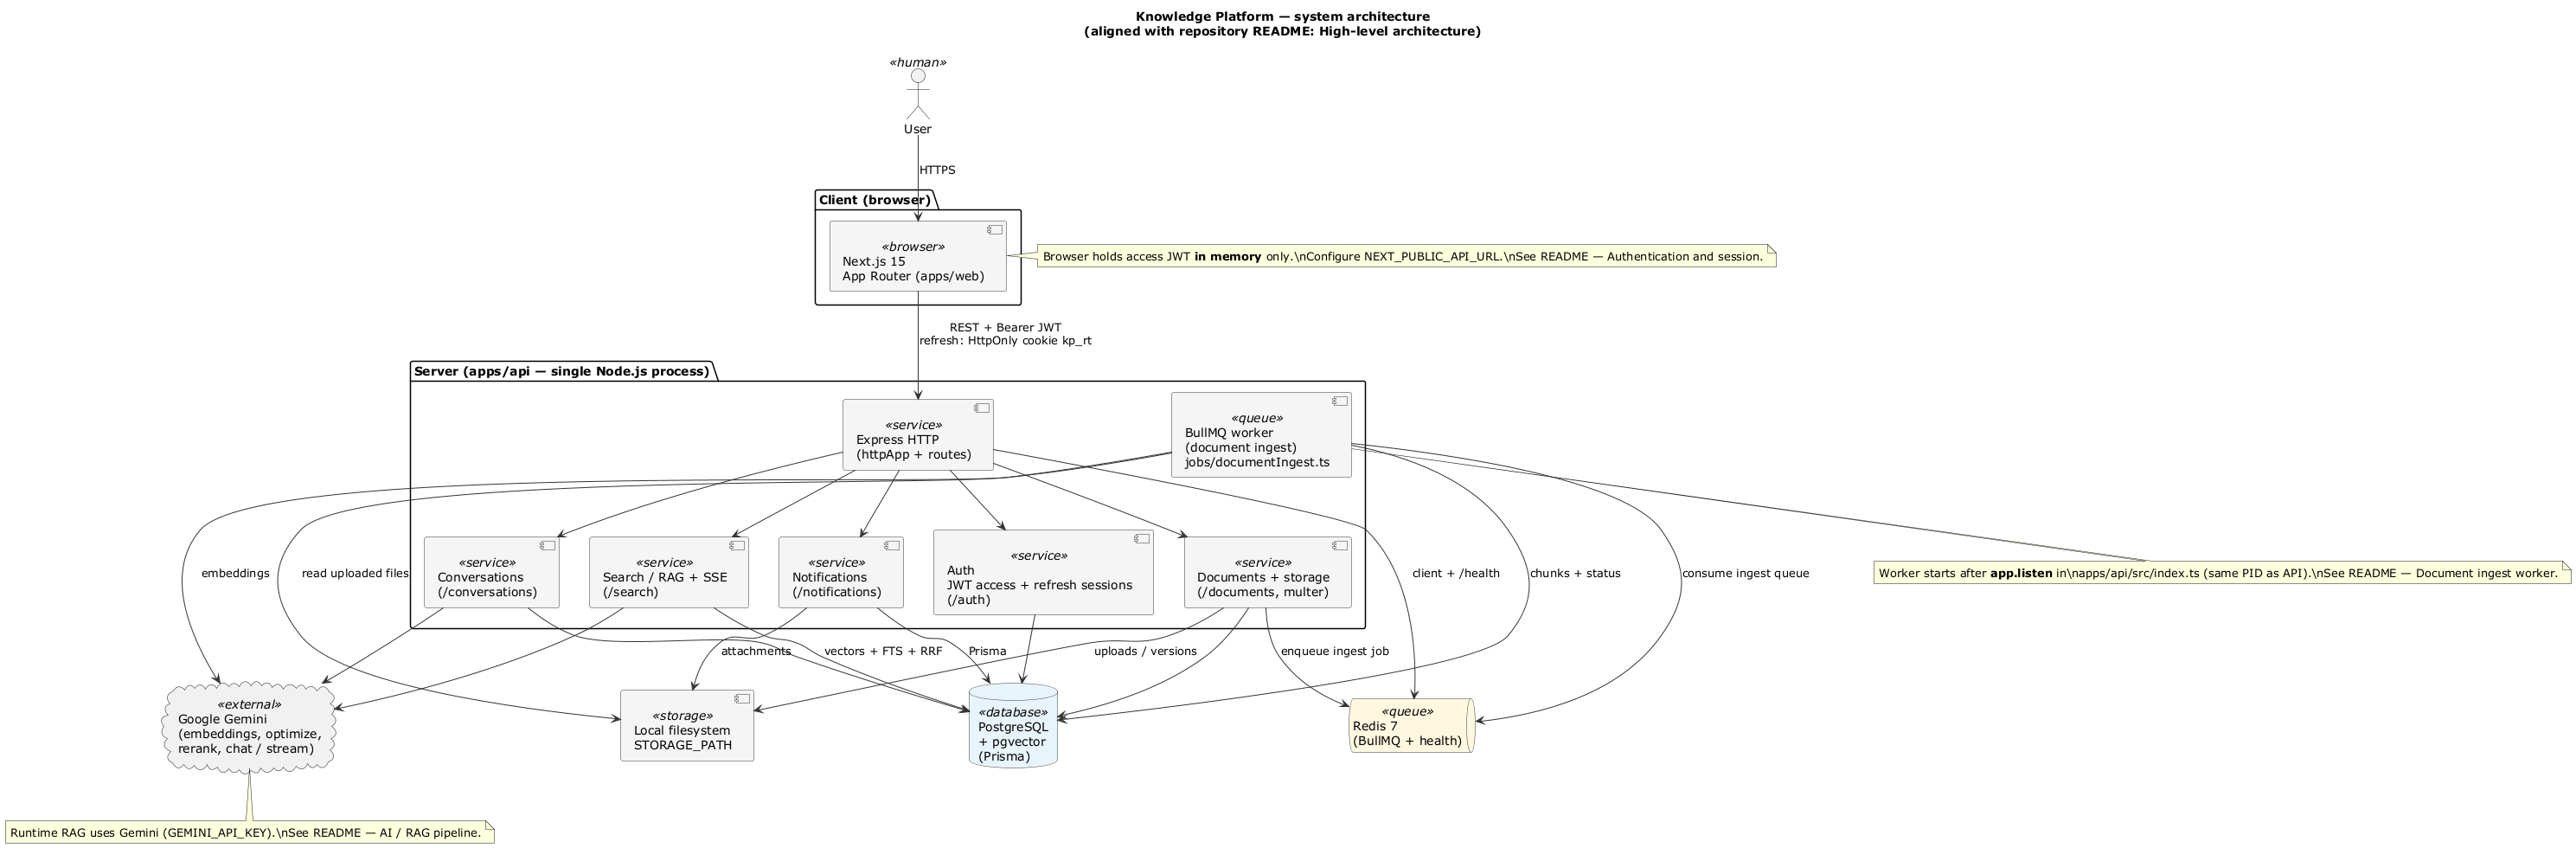
\includegraphics[width=0.98\textwidth]{assets/figures/platform-architecture.png}
\caption[Overall platform architecture]{Overall architecture of the Knowledge Platform (PlantUML source: \texttt{platform-architecture.puml})}
\label{fig:architecture}
\end{figure}

The web application (\texttt{apps/web}) keeps access tokens in memory and uses HttpOnly refresh cookies. The API (\texttt{apps/api}) mounts routers for \texttt{/auth}, \texttt{/documents}, \texttt{/search}, \texttt{/conversations}, \texttt{/admin}, \texttt{/manager}, \texttt{/notifications}, and public \texttt{/avatars}. A BullMQ consumer runs in the same Node process after the HTTP server starts.

\section{Logical Subsystem Decomposition}
\label{sec:subsystem-decomposition}

\begin{table}[H]
\centering
\caption{Subsystem responsibilities}
\label{tab:subsystems}
\renewcommand{\arraystretch}{1.35}
\begin{tabularx}{\textwidth}{|>{\RaggedRight\arraybackslash}p{2.5cm}|Y|>{\RaggedRight\arraybackslash}p{3.1cm}|}
\hline
\rowcolor{sectionblue!15}
\textbf{Subsystem} & \textbf{Responsibility} & \textbf{Key modules} \\
\hline
Authentication & Login, refresh families, restrictions, password reset &
\tcodelines{auth.ts}{authClient.ts} \\
\hline
Documents & CRUD, versions, visibility, audit, download &
\tcodelines{documents.ts}{storage.ts} \\
\hline
Ingest worker & Extract, chunk, embed, persist chunks &
\tcodelines{BullMQ worker}{index.ts} \\
\hline
Search / RAG & Hybrid retrieval, SSE answers, cache &
\tcodelines{search.ts}{ragCompletion.ts} \\
\hline
Conversations & Threads, messages, feedback &
\tcode{conversations.ts} \\
\hline
Notifications & Auto events and manual announcements &
\tcode{notifications.ts} \\
\hline
Admin / Manager & Governance dashboards &
\tcodelines{admin.ts}{manager.ts} \\
\hline
\end{tabularx}
\end{table}

\section{Domain Data Model}
\label{sec:domain-model}

The Prisma schema defines 20+ entities including \texttt{User}, \texttt{Department},
\texttt{Document}, \texttt{DocumentVersion}, \texttt{Chunk} (768-d embedding),
\texttt{Conversation}, \texttt{AnswerFeedback}, and \texttt{Notification}.
Multi-department access is modeled through \texttt{UserDepartmentAccess}.
Figure~\ref{fig:class-diagram} presents the principal persisted classes and their
relationships across all sprints; sprint-scoped excerpts appear in
Section~\ref{sec:sprint-design}.

\begin{figure}[H]
\centering
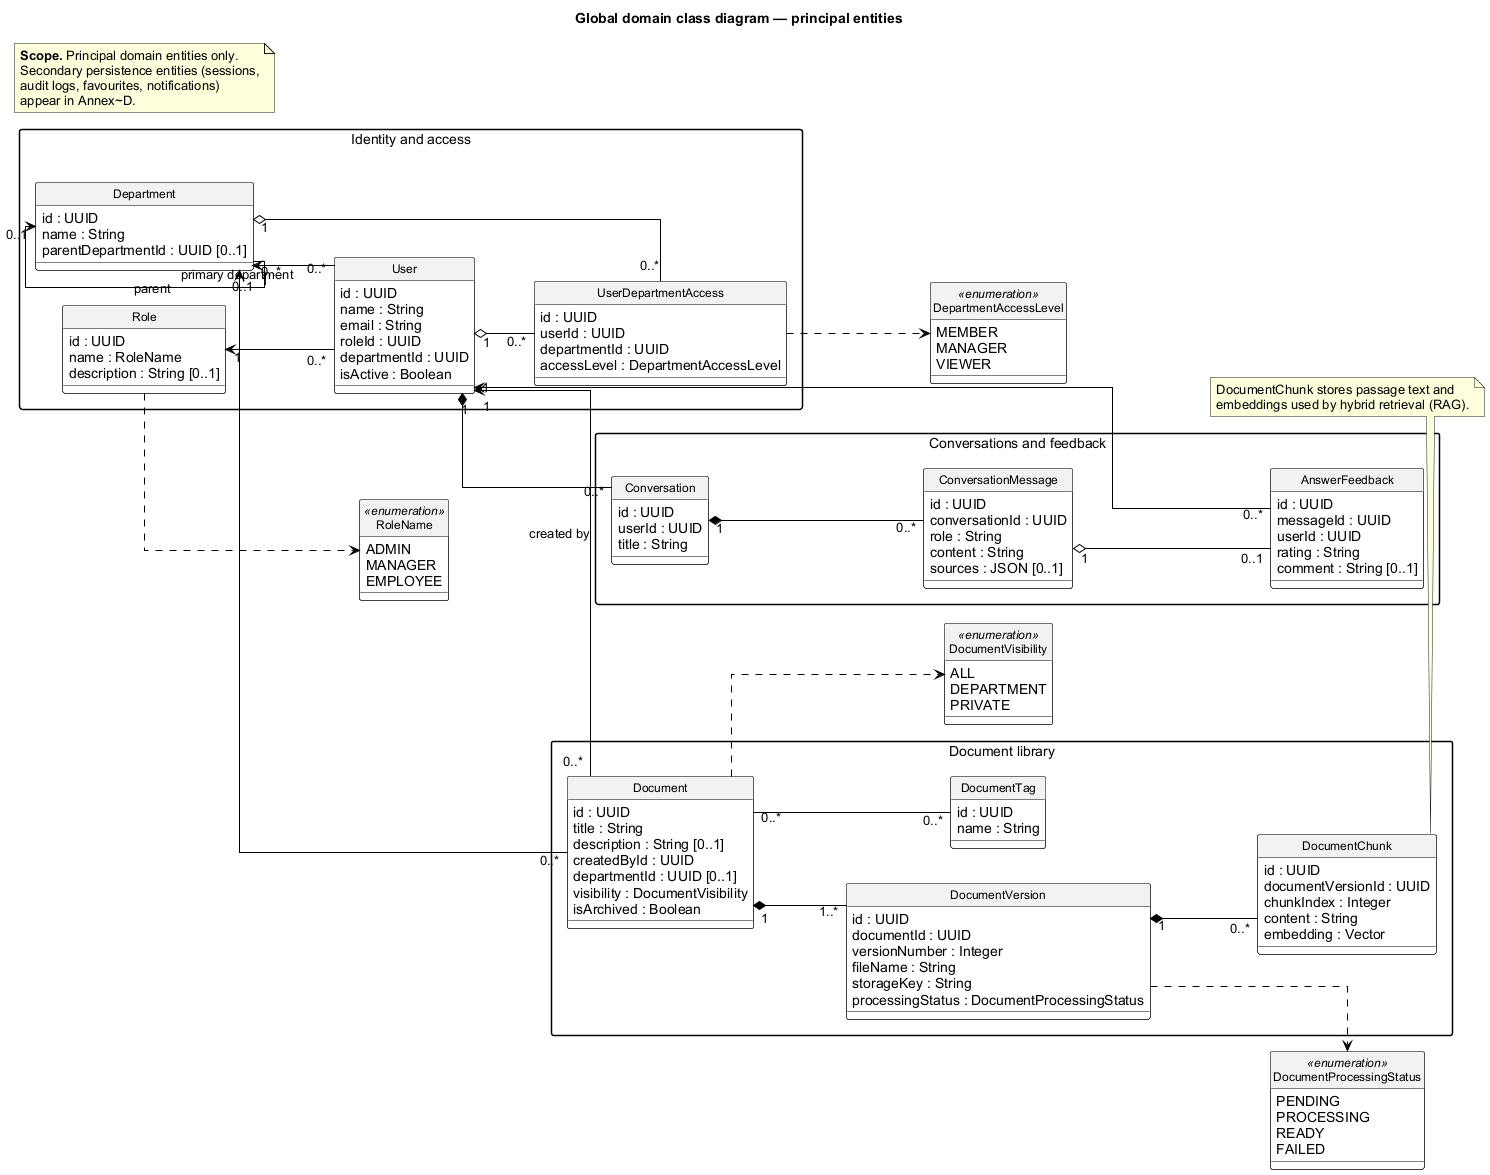
\includegraphics[width=0.98\textwidth,keepaspectratio]{assets/figures/global-class-knowledge-platform.png}
\caption{Global domain class diagram (persisted entities and main relationships)}
\label{fig:class-diagram}
\end{figure}

\section{Technology Choice Justification}
\label{sec:technology-justification}

Table~\ref{tab:decision-matrix} scores architectural options (1 = weak, 3 = strong).
The selected stack favours a TypeScript monorepo with Express and Next.js for
streaming RAG, operational simplicity, and alignment with project skills.

\begin{table}[H]
\centering
\caption{Decision-support matrix for platform architecture (scores: 1 = weak, 3 = strong)}
\label{tab:decision-matrix}
\renewcommand{\arraystretch}{1.4}
\setlength{\tabcolsep}{5pt}
\begin{tabularx}{\textwidth}{|>{\RaggedRight\arraybackslash}p{2.6cm}|>{\Centering\arraybackslash}p{1.7cm}|>{\Centering\arraybackslash}p{1.3cm}|>{\Centering\arraybackslash}p{2.1cm}|Y|}
\hline
\rowcolor{sectionblue!15}
\textbf{Criterion} &
\textbf{Monorepo} &
\textbf{Django} &
\textbf{Microservices} &
\textbf{Rationale} \\
\hline
Time to market & 3 & 2 & 1 & Shared TypeScript types; one repository \\
\hline
SSE streaming fit & 3 & 2 & 2 & Native Express streaming for RAG \\
\hline
Team skill alignment & 3 & 2 & 1 & Matches React + Node stack \\
\hline
Operational complexity & 3 & 3 & 1 & Single API process + worker \\
\hline
\end{tabularx}
\end{table}

\textbf{PostgreSQL + pgvector vs.\ dedicated vector DB:} colocating relational and vector data simplifies hybrid SQL+vector retrieval, transactional consistency, and department filters in one query layer~\cite{pgvector-docs}.

\textbf{Gemini vs.\ open-weight models:} the embedding and chat APIs reduce operational burden while providing strong multilingual embeddings (768 dimensions in this deployment)~\cite{google-gemini-docs}.

\textbf{In-process BullMQ worker vs.\ separate worker service:} embedding the consumer in the API process reduces deployment complexity for an academic/prototype-scale platform, at the cost of horizontal scaling coupling.

Table~\ref{tab:traceability-main} links representative requirements to the chosen
design elements and validation artefacts (see also Table~\ref{tab:fr-traceability}
in Chapter~\ref{ch:requirements}).

\begin{table}[H]
\centering
\caption{Requirements-to-design traceability (excerpt)}
\label{tab:traceability-main}
\footnotesize
\renewcommand{\arraystretch}{1.35}
\setlength{\tabcolsep}{4pt}
\begin{tabularx}{\textwidth}{|>{\RaggedRight\arraybackslash}p{1.0cm}|>{\RaggedRight\arraybackslash}p{2.5cm}|Y|>{\RaggedRight\arraybackslash}p{2.6cm}|}
\hline
\rowcolor{sectionblue!15}
\textbf{Req.} & \textbf{Design choice} & \textbf{Implemented element} & \textbf{Validation} \\
\hline
FR-01 & JWT + refresh rotation &
\tcodelines{auth.ts}{authClient.ts} &
\testfile{auth.integration.test} \\
\hline
FR-02 & Avatar CORP header &
\tcode{avatarsPublic.ts} &
\testfile{avatars.integration.test} \\
\hline
FR-03 & Async ingest queue &
\tcode{BullMQ + Redis} &
\testfile{documents.integration.test} \\
\hline
FR-07 & Hybrid RAG + SSE &
\tcodelines{search.ts}{ragCompletion.ts} &
\testfile{search.integration.test} \\
\hline
FR-10 & Admin RBAC &
\tcode{admin.ts} &
\testfile{admin.integration.test} \\
\hline
NFR-02 & Helmet + rate limits &
\tcode{httpApp.ts} &
manual + integration \\
\hline
\end{tabularx}
\end{table}

\section{Dynamic Interaction Design by Sprint}
\label{sec:sprint-design}

Sections~\ref{sec:overall-architecture}--\ref{sec:technology-justification} describe
\textbf{what} the platform is made of (components, data, and technology). This section
describes \textbf{how} actors and subsystems interact at runtime. For each sprint in
Table~\ref{tab:sprints} of Chapter~\ref{ch:requirements}, the design is organised in
three layers:
\begin{enumerate}[leftmargin=*,itemsep=0.2em]
  \item \textbf{Sprint scope} --- objectives and mapped functional requirements;
  \item \textbf{Scoped structural views} --- sprint use-case model and sprint domain class model;
  \item \textbf{Interaction sequence diagrams} --- request/response flows between client, API, workers, and external services.
\end{enumerate}
The full diagram catalog is indexed in Appendix~\ref{annex:diagrams}; implementation
evidence appears in Chapter~\ref{ch:implementation} and validation in
Chapter~\ref{ch:validation}.

\subsection{Sprint 1: Authentication and access control}\label{subsec:sprint1-design}

Sprint~1 establishes the security perimeter of the platform. It delivers
credential-based authentication with refresh-token rotation (FR-01), profile and
avatar management (FR-02), per-user feature restrictions (FR-12), and the
non-functional controls for HTTP hardening and single-flight token refresh
(NFR-02, NFR-03).

\sprintstructural{1}%
  {Sprint 1 use-case diagram — Authentication and access control}{fig:sprint1-use-cases}%
  {Sprint 1 domain class diagram — Authentication and access control}{fig:sprint1-class}

\sprintsequences{1}

\sprintflowgroup{Authentication and session management}

\paragraph{User login.}
The login flow validates email and password against bcrypt hashes, enforces account
lockout after repeated failures, and issues a short-lived access JWT together with
an HttpOnly refresh cookie bound to a token family stored in the database.
\seqdiagram{seq-01-login}{User login}{POST /auth/login}{fig:seq-01}

\paragraph{Access token refresh and session rotation.}
When the in-memory access token expires, the web client triggers a single
in-flight refresh request that rotates the refresh cookie, invalidates the
previous family member, and returns a new access token without user interaction.
\seqdiagram{seq-02-refresh-token}{Access token refresh and session rotation}{POST /auth/refresh}{fig:seq-02}

\paragraph{User logout.}
Logout revokes the active refresh-token family server-side and clears the
HttpOnly cookie, ensuring that stolen refresh tokens cannot be reused after the
user explicitly ends the session.
\seqdiagram{seq-03-logout}{User logout}{POST /auth/logout}{fig:seq-03}

\paragraph{Forgot and reset password.}
Password recovery sends a time-limited reset link by email; the reset endpoint
validates the token, applies the password policy, and invalidates all outstanding
refresh families for the affected account.
\seqdiagram{seq-04-password-reset}{Forgot and reset password}{POST /auth/forgot-password, reset-password}{fig:seq-04}

\paragraph{Change password with session invalidation.}
Authenticated users may change their password by supplying the current secret;
successful rotation updates the hash, enforces policy rules, and terminates other
active sessions through family revocation.
\seqdiagram{seq-05-change-password}{Change password with session invalidation}{POST /auth/change-password}{fig:seq-05}

\sprintflowgroup{Profile, restrictions and session context}

\paragraph{Profile update.}
Profile updates accept display name and avatar file uploads; the API persists
metadata in Prisma and stores avatar binaries on disk, exposing them through the
public \texttt{/avatars} route with cross-origin headers.
\seqdiagram{seq-06-profile-update}{Profile update}{PATCH /auth/profile}{fig:seq-06}

\paragraph{Feature restriction enforcement.}
Middleware consults per-user feature flags before protected handlers execute;
restricted users receive a structured \texttt{403 FEATURE\_RESTRICTED} response
that the web client maps to a dedicated explanation page.
\seqdiagram{seq-07-feature-restriction}{Feature restriction enforcement}{403 FEATURE\_RESTRICTED}{fig:seq-07}

\paragraph{Current user session payload.}
The \texttt{/me} endpoint returns the authenticated principal, role, department
memberships, and active feature restrictions so the client can render navigation
and gate UI affordances without additional round trips.
\seqdiagram{seq-23-get-auth-me}{Current user session payload}{GET /auth/me}{fig:seq-23}

\sprintflowgroup{Guest and restricted UX pages}

\paragraph{Register information page (no self-service signup).}
Self-service registration is intentionally disabled; the static \texttt{/register}
page informs visitors that accounts are provisioned by administrators, avoiding
orphan users outside the RBAC model.
\seqdiagram{seq-32-register-info-static}{Register information page (no self-service signup)}{Next.js /register}{fig:seq-32}

\paragraph{Restricted feature explanation page.}
When the API signals a feature restriction, the client redirects to
\texttt{/restricted}, presenting context-sensitive guidance rather than a generic
error banner.
\seqdiagram{seq-33-restricted-page-ux}{Restricted feature explanation page}{/restricted UX}{fig:seq-33}

\subsection{Sprint 2: Document library and ingest}\label{subsec:sprint2-design}

Sprint~2 implements the document corpus lifecycle: multi-format upload and storage
(FR-03), department-scoped visibility enforcement (FR-04), and library
organisation features such as versioning, tags, favorites, and recents (FR-05).
Uploads are accepted synchronously by the API while text extraction, chunking, and
embedding run asynchronously in a BullMQ worker.

\sprintstructural{2}%
  {Sprint 2 use-case diagram — Document library and ingest}{fig:sprint2-use-cases}%
  {Sprint 2 domain class diagram — Document library and ingest}{fig:sprint2-class}

\sprintsequences{2}

\sprintflowgroup{Upload and asynchronous ingest}

\paragraph{Document upload.}
The upload endpoint validates MIME type and size, writes the binary to disk,
creates \texttt{Document} and \texttt{DocumentVersion} rows, and enqueues an
ingest job keyed by version identifier.
\seqdiagram{seq-08-document-upload}{Document upload}{POST /documents/upload}{fig:seq-08}

\paragraph{Asynchronous ingest worker.}
The BullMQ consumer loads the stored file, extracts text per format, splits
content into sentence-aware chunks with table preservation, computes
768-dimensional embeddings, and persists \texttt{Chunk} rows indexed for retrieval.
\seqdiagram{seq-09-document-ingest-worker}{Asynchronous ingest worker}{BullMQ processIngest}{fig:seq-09}

\paragraph{Reprocess document version.}
Administrators can force re-ingestion of an existing version---for example after
embedding model upgrades---without re-uploading the binary.
\seqdiagram{seq-29-document-reprocess}{Reprocess document version}{POST .../reprocess}{fig:seq-29}

\sprintflowgroup{Library access and download}

\paragraph{Document file download.}
Authorized users download the original file through a version-scoped endpoint that
re-checks department visibility before streaming bytes from the storage backend.
\seqdiagram{seq-10-document-read-download}{Document file download}{GET .../file}{fig:seq-10}

\paragraph{Document list.}
The list endpoint applies department filters, search facets, and pagination,
returning summary metadata suitable for the library grid without loading chunk
payloads.
\seqdiagram{seq-24-documents-list}{Document list}{GET /documents}{fig:seq-24}

\paragraph{Document detail.}
Detail retrieval joins document metadata, active version, tags, ingest status, and
audit hints, giving the preview pane everything required for inline viewing.
\seqdiagram{seq-25-document-detail}{Document detail}{GET /documents/:id}{fig:seq-25}

\paragraph{Favorites and recents.}
Users pin documents to favorites and the API records recent views; both features
are scoped to the authenticated principal and surfaced on the library home view.
\seqdiagram{seq-26-favorites-recents}{Favorites and recents}{POST/DELETE favorite, recent view}{fig:seq-26}

\sprintflowgroup{Metadata and versioning}

\paragraph{Document metadata update.}
Managers and owners may patch title, description, tags, and visibility; changes
are validated against writable department scopes and written to the audit trail.
\seqdiagram{seq-27-patch-document-metadata}{Document metadata update}{PATCH /documents/:id}{fig:seq-27}

\paragraph{New document version.}
Uploading a replacement file creates a new \texttt{DocumentVersion}, triggers a
fresh ingest job, and keeps prior versions available for rollback and audit.
\seqdiagram{seq-28-document-new-version}{New document version}{POST /documents/:id/versions}{fig:seq-28}

\subsection{Sprint 3: Search, RAG and conversations}\label{subsec:sprint3-design}

Sprint~3 delivers the intelligent retrieval layer: semantic search over embedded
chunks (FR-06), hybrid retrieval-augmented generation with streaming answers
(FR-07), and persistent conversation threads with feedback (FR-08). The RAG
evaluation harness (NFR-06) is introduced in parallel to measure answer quality
against golden datasets.

\sprintstructural{3}%
  {Sprint 3 use-case diagram — Search, RAG and conversations}{fig:sprint3-use-cases}%
  {Sprint 3 domain class diagram — Search, RAG and conversations}{fig:sprint3-class}

\sprintsequences{3}

\sprintflowgroup{Search and hybrid RAG}

\paragraph{Semantic vector search.}
The semantic search endpoint embeds the user query, queries pgvector with
department filters, and returns ranked chunks with snippet previews for quick
exploration outside the chat UI.
\seqdiagram{seq-11-semantic-search}{Semantic vector search}{POST /search/semantic}{fig:seq-11}

\paragraph{Hybrid RAG Ask with SSE streaming.}
The Ask endpoint orchestrates query optimisation, dense and sparse retrieval,
reciprocal-rank fusion, LLM reranking, and streams tokens plus source citations
to the browser over Server-Sent Events.
\seqdiagram{seq-12-ask-rag-sse}{Hybrid RAG Ask with SSE streaming}{POST /search/ask}{fig:seq-12}

\sprintflowgroup{Conversations and answer quality}

\paragraph{Conversation and messages.}
Users create conversation threads, append questions, and retrieve message history;
each assistant turn stores retrieved sources, confidence metadata, and links back
to originating chunks.
\seqdiagram{seq-13-conversation-and-messages}{Conversation and messages}{/conversations}{fig:seq-13}

\paragraph{Answer feedback.}
After each answer, users may submit thumbs-up/down feedback with optional comments;
the API persists \texttt{AnswerFeedback} rows used later for quality dashboards.
\seqdiagram{seq-14-answer-feedback}{Answer feedback}{POST .../feedback}{fig:seq-14}

\paragraph{Conversation CRUD supplement.}
Beyond the primary messaging flow, clients list, rename, and delete conversations
through supplementary endpoints that keep thread metadata consistent with UI state.
\seqdiagram{seq-30-conversations-crud-supplement}{Conversation CRUD supplement}{list, patch, delete}{fig:seq-30}

\paragraph{Admin feedback statistics.}
Administrators query aggregated feedback metrics---volume, sentiment ratio, and
recent comments---to monitor RAG quality trends across departments.
\seqdiagram{seq-31-admin-feedback-stats}{Admin feedback statistics}{GET /conversations/feedback/stats}{fig:seq-31}

\subsection{Sprint 4: Governance and notifications}\label{subsec:sprint4-design}

Sprint~4 covers organisational governance: automatic and manual notifications
(FR-09), administrator tooling for users, departments, and bulk operations
(FR-10), and the manager department dashboard (FR-11). Notification events are
decoupled from document mutations through a service layer, while admin routes
enforce elevated RBAC and emit structured audit records for every destructive
action.

\sprintstructural{4}%
  {Sprint 4 use-case diagram — Governance and notifications}{fig:sprint4-use-cases}%
  {Sprint 4 domain class diagram — Governance and notifications}{fig:sprint4-class}

\sprintsequences{4}

\sprintflowgroup{Notification subsystem}

\paragraph{Automatic notification on document events.}
When documents are created or materially updated, the notification service fans
out inbox entries to subscribed department members without blocking the upload
response path.
\seqdiagram{seq-15-notification-automatic}{Automatic notification on document events}{notifyDocumentCreated}{fig:seq-15}

\paragraph{Manual announcement.}
Administrators compose announcements with optional attachments; the send endpoint
validates audience scope and delivers messages to targeted user inboxes.
\seqdiagram{seq-16-notification-manual-send}{Manual announcement}{POST /notifications/send}{fig:seq-16}

\paragraph{Notification inbox.}
Users list notifications, query unread counts, mark items as read, and download
attachments through REST endpoints polled by the web shell.
\seqdiagram{seq-17-notification-inbox}{Notification inbox}{list, unread, mark read, attachment}{fig:seq-17}

\sprintflowgroup{Manager dashboard}

\paragraph{Manager department overview.}
Managers retrieve department-scoped KPIs---document counts, recent activity, and
team membership---through dedicated \texttt{/manager} routes filtered to
manageable departments.
\seqdiagram{seq-18-manager-dashboard}{Manager department overview}{GET /manager/*}{fig:seq-18}

\sprintflowgroup{Administrator governance}

\paragraph{Admin create user.}
Administrators provision accounts with initial roles, department assignments, and
optional feature restrictions; credentials are communicated out-of-band per
organisational policy.
\seqdiagram{seq-19-admin-user-create}{Admin create user}{POST /admin/users}{fig:seq-19}

\paragraph{Admin merge departments.}
Department merge consolidates documents, access grants, and memberships from a
source department into a target, preserving referential integrity inside a
transaction.
\seqdiagram{seq-20-admin-department-merge}{Admin merge departments}{POST /admin/departments/merge}{fig:seq-20}

\paragraph{Bulk department access.}
Bulk PUT replaces the full access matrix for a user or department in one request,
simplifying onboarding scripts and CSV-driven imports.
\seqdiagram{seq-21-admin-department-access-bulk}{Bulk department access}{PUT .../department-access}{fig:seq-21}

\paragraph{Admin create department.}
New organisational units are created with unique slugs; the operation is restricted
to administrators and is logged for compliance review.
\seqdiagram{seq-34-admin-department-create}{Admin create department}{POST /admin/departments}{fig:seq-34}

\paragraph{Single department access grant/revoke.}
Fine-grained POST and DELETE endpoints add or remove individual department access
rows without rewriting the entire access matrix.
\seqdiagram{seq-35-dept-access-single-post-delete}{Single department access grant/revoke}{POST/DELETE access}{fig:seq-35}

\paragraph{Admin KPI statistics.}
The admin statistics endpoint aggregates platform-wide counters---users,
documents, conversations, and ingest backlog---for dashboard cards.
\seqdiagram{seq-36-admin-stats}{Admin KPI statistics}{GET /admin/stats}{fig:seq-36}

\paragraph{Admin activity log and CSV export.}
Administrators browse paginated activity logs and export filtered events to CSV for
offline analysis, with formula-injection escaping on downloadable fields.
\seqdiagram{seq-37-admin-activity-export}{Admin activity log and CSV export}{GET /admin/activity}{fig:seq-37}

\paragraph{Document audit trail.}
Per-document audit views expose who changed metadata, visibility, or versions,
supporting forensic review during access reviews.
\seqdiagram{seq-38-admin-document-audit}{Document audit trail}{GET /admin/document-audit}{fig:seq-38}

\paragraph{Documents CSV export.}
Administrators export the document catalogue---titles, departments, tags, and ingest
status---as CSV for inventory reconciliation.
\seqdiagram{seq-39-admin-documents-csv-export}{Documents CSV export}{GET /documents/export}{fig:seq-39}

\paragraph{Bulk document delete.}
Bulk delete accepts a list of document identifiers, verifies administrator scope,
removes storage artefacts, and cascades database rows inside a guarded transaction.
\seqdiagram{seq-40-admin-bulk-delete-documents}{Bulk document delete}{POST /documents/bulk-delete}{fig:seq-40}

\paragraph{Admin user patch and lock.}
Administrators update user roles, restrictions, and lock state; account lock
immediately invalidates refresh families to block further API access.
\seqdiagram{seq-41-admin-user-patch-lock}{Admin user patch and lock}{PATCH/lock user}{fig:seq-41}

\subsection{Sprint 5: Operations, testing and deployment}\label{subsec:sprint5-design}

Sprint~5 hardens operability and reproducibility: a public health probe (NFR-01),
containerised deployment (NFR-04), a broad integration-test suite (NFR-05), and
the RAG evaluation harness (NFR-06). Unlike feature sprints, several deliverables
are cross-cutting quality gates rather than user-visible flows.

\sprintstructural{5}%
  {Sprint 5 use-case diagram — Operations, testing and deployment}{fig:sprint5-use-cases}%
  {Sprint 5 domain class diagram — Operations, testing and deployment}{fig:sprint5-class}

\sprintsequences{5}

\paragraph{API health probe.}
Load balancers and orchestrators call \texttt{GET /health} to verify that the API
process is running and can reach PostgreSQL and Redis; the endpoint returns a
compact JSON status without authentication.
\seqdiagram{seq-22-health-check}{API health probe}{GET /health}{fig:seq-22}

\subsubsection{Operational deliverables}
\label{subsubsec:sprint5-operations}

\paragraph{Integration test suite.}
The API ships with a Vitest and Supertest integration suite spanning
authentication, documents, search, conversations, admin, and manager routers.
Tests spin up an isolated database schema, seed fixtures, and assert HTTP
contracts against the same routes documented in the sequence diagrams above,
providing regression coverage for NFR-05.

\paragraph{Docker Compose deployment.}
Production-oriented Compose files package the API, web, PostgreSQL with pgvector,
and Redis behind documented environment variables and volume mounts. Migrations run
through the Prisma CLI inside the API container, ensuring that any workstation
or CI agent can reproduce the full stack with a single \texttt{docker compose up}
invocation (NFR-04).

\paragraph{RAG evaluation harness.}
A command-line evaluation harness loads golden question--answer pairs, invokes the
Ask pipeline programmatically, and scores responses with an automated LLM judge.
Reports are written to \texttt{eval-reports/} so retrieval prompt changes can be
compared across commits, fulfilling the reproducible quality gate of NFR-06.


\section{Chapter Conclusion}

This chapter defined the architectural foundation of the Knowledge Platform in two
complementary views: static design (architecture, subsystems, domain model, and
technology justification) and dynamic design (sprint-scoped structural views and
interaction sequence diagrams). The decision matrix and requirements-to-design
traceability established that each major functional and non-functional requirement
is mapped to concrete modules, interaction flows, and validation evidence.
Chapter~\ref{ch:implementation} describes how these design artefacts were realized
in code.

\chapter[Implementation]{Realization, implementation or experimentation}
\label{ch:implementation}

This chapter describes how the sprint-aligned design of
Section~\ref{sec:sprint-design} (Chapter~\ref{ch:architecture}) was realized in
code. Implementation follows the five-sprint plan of Table~\ref{tab:sprints},
with each subsection summarising the principal modules, technical choices, and
sequence flows validated for that increment.

\section{Hardware and Software Environment}

\begin{table}[H]
\centering
\caption{Development and deployment stack}
\label{tab:stack}
\begin{tabularx}{\textwidth}{>{\RaggedRight\arraybackslash}p{2.8cm} Y}
\toprule
Layer & Technology (versions) \\
\midrule
Workstation & Windows 10/11; Node.js 20+ \\
API & Express 4, TypeScript, Prisma 5, Vitest 3 \\
Web & Next.js 15, React 19, CSS Modules \\
Database & PostgreSQL 16 with pgvector extension \\
Queue & Redis 7, BullMQ 5 \\
AI services & Google Gemini (\tcode{gemini-2.5-flash}, \tcode{gemini-embedding-001}) \\
Containers & Docker Compose (dev and prod compose files) \\
\bottomrule
\end{tabularx}
\end{table}

The monorepo root orchestrates \texttt{npm run dev} (API on port 3001, web on 3000), database migrations, seeding, linting, and RAG evaluation scripts.

\section{Implementation Steps by Sprint}

\subsection{Sprint 1: Authentication and access control}
\label{subsec:impl-sprint1}

Sprint~1 implements the security perimeter defined in
Subsection~\ref{subsec:sprint1-design} (FR-01, FR-02, FR-12; NFR-02, NFR-03).
Access tokens are short-lived JWTs stored \textbf{in memory} on the web client---never
in \texttt{localStorage}---to reduce XSS exfiltration risk. Refresh tokens live in
HttpOnly cookies (\texttt{kp\_rt}). The client uses a \textbf{single in-flight}
refresh promise to prevent parallel rotations from invalidating each other~\cite{ietf-jwt-bcp}.
Role middleware and per-user restriction flags (\tcode{requireDocLibraryAccess},
\tcode{requireUseAiQueries}) enforce the hybrid authorization model of
Subsection~\ref{subsec:access-control-model}. Profile avatars are served from a
CORP-aware public route (\tcode{avatarsPublic.ts}). Flows
\ref{fig:seq-01}--\ref{fig:seq-07}, \ref{fig:seq-23}, \ref{fig:seq-32}, and
\ref{fig:seq-33} were validated against integration tests in
\tcode{auth.integration.test} and \tcode{avatars.integration.test}.

\subsection{Sprint 2: Document library and ingest pipeline}
\label{subsec:impl-sprint2}

Sprint~2 delivers the document lifecycle of Subsection~\ref{subsec:sprint2-design}
(FR-03 to FR-05). Uploads are validated (MIME allowlist, size limits), stored on
disk, and enqueued in BullMQ. The worker extracts text per format (PDF, Office,
HTML, etc.), chunks content with sentence-aware splitting and table preservation,
computes 768-dimensional embeddings, and persists \texttt{Chunk} rows with vector
indexes. Visibility rules (\texttt{ALL}, \texttt{DEPARTMENT}, \texttt{PRIVATE}) are
enforced through \tcode{canReadDocument} in \tcode{documentAccess.ts}, returning
404 on unauthorised access to prevent enumeration. Tags, favorites, recents, and
versioning are handled in \tcode{documents.ts}. Flows
\ref{fig:seq-08}--\ref{fig:seq-10} and \ref{fig:seq-24}--\ref{fig:seq-29} are
covered by \tcode{documents.integration.test}.

\subsection{Sprint 3: Search, RAG and conversations}
\label{subsec:impl-sprint3}

Sprint~3 implements the hybrid retrieval and AI assistant of
Subsection~\ref{subsec:sprint3-design} (FR-06 to FR-08; NFR-06).
Algorithm~\ref{alg:rag} summarizes the Ask endpoint logic in
\tcode{search.ts} and \tcode{ragCompletion.ts}.

\begin{algorithm}[H]
\caption{Hybrid RAG Ask pipeline (simplified)}
\label{alg:rag}
\begin{algorithmic}[1]
\State Authenticate user and resolve \texttt{readableDepartmentIds}
\State Optimize query (type, topic, rewrite, optional multi-hop)
\State Retrieve dense vectors (pgvector) and sparse FTS (BM25-style)
\State Fuse rankings with weighted reciprocal rank fusion (RRF)
\State Rerank top chunks with Gemini; optionally expand neighbor chunks
\State Stream SSE events: \texttt{sources}, \texttt{token}, optional \texttt{correction}
\State Persist conversation message with citations and confidence
\State Optionally cache answer keyed by prompt version and filters
\end{algorithmic}
\end{algorithm}

The Ask UI consumes SSE streams and renders markdown with sanitized links.
Conversation threads, message persistence, and thumbs-up/down feedback are
implemented in \tcode{conversations.ts}. Semantic search and Ask flows
(\ref{fig:seq-11}, \ref{fig:seq-12}) plus conversation sequences
(\ref{fig:seq-13}, \ref{fig:seq-14}, \ref{fig:seq-30}, \ref{fig:seq-31}) are
validated in \tcode{search.integration.test} and
\tcode{conversations.integration.test}.

\subsection{Sprint 4: Governance and notifications}
\label{subsec:impl-sprint4}

Sprint~4 covers administration, manager dashboards, and notifications per
Subsection~\ref{subsec:sprint4-design} (FR-09 to FR-11).
\texttt{departmentAccess.ts} computes readable and manageable department sets
including inherited manager/viewer scopes. Administrators manage users, bulk
restrictions, CSV import (with formula-injection escaping), department merge, KPI
exports, and document audit views in \tcode{admin.ts}. Managers access
department-scoped dashboards through \tcode{manager.ts}. The notification service
emits automatic events on document lifecycle changes and supports manual
announcements with attachments. Document previews use blob URLs for PDF/images;
notifications use polling with unread badges. Admin, manager, and notification
flows (\ref{fig:seq-15}--\ref{fig:seq-21}, \ref{fig:seq-34}--\ref{fig:seq-41})
are covered by \tcode{admin.integration.test}, \tcode{manager.integration.test},
and \tcode{notifications.integration.test}.

\subsection{Sprint 5: Operations, testing and deployment}
\label{subsec:impl-sprint5}

Sprint~5 consolidates operational readiness per
Subsection~\ref{subsec:sprint5-design} (NFR-01, NFR-04 to NFR-06). The health
probe (\ref{fig:seq-22}) reports PostgreSQL and Redis status via
\tcode{GET /health}. A 74-test Vitest/Supertest suite runs against real database
and Redis instances (\texttt{npm run test:api}). Docker Compose files provide
reproducible dev and production stacks with automatic migrations. The RAG
evaluation CLI (\texttt{npm run eval:rag:quick}, \texttt{npm run eval:rag})
writes JSON reports under \texttt{eval-reports/}. Table~\ref{tab:seq-index}
summarises all sprint sequence flows; the complete catalog appears in
Appendix~\ref{annex:diagrams} (Table~\ref{tab:annex-seq-index}).

\begin{table}[H]
\centering
\caption{Index of implementation sequence diagrams (Chapter~\ref{ch:architecture}, \S\ref{sec:sprint-design})}
\label{tab:seq-index}
\scriptsize
\begin{tabularx}{\textwidth}{|>{\Centering\arraybackslash}p{0.8cm}|>{\RaggedRight\arraybackslash}p{2.3cm}|>{\Centering\arraybackslash}p{1.0cm}|Y|}
\hline
\rowcolor{sectionblue!15}
\textbf{Sprint} & \textbf{Area} & \textbf{Fig.} & \textbf{Flow} \\
\hline
S1 & Auth & \ref{fig:seq-01}--\ref{fig:seq-07}, \ref{fig:seq-23}, \ref{fig:seq-32}, \ref{fig:seq-33} & Login, refresh, logout, password reset/change, profile, restrictions, /me, register info, restricted UX \\
\hline
S2 & Documents & \ref{fig:seq-08}--\ref{fig:seq-10}, \ref{fig:seq-24}--\ref{fig:seq-29} & Upload, ingest worker, download, list, detail, favorites, metadata, versions, reprocess \\
\hline
S3 & Search / RAG & \ref{fig:seq-11}, \ref{fig:seq-12} & Semantic search, hybrid Ask SSE \\
\hline
S3 & Conversations & \ref{fig:seq-13}, \ref{fig:seq-14}, \ref{fig:seq-30}, \ref{fig:seq-31} & Threads, messages, feedback, CRUD supplement, admin stats \\
\hline
S4 & Notifications & \ref{fig:seq-15}--\ref{fig:seq-17} & Automatic events, manual send, inbox \\
\hline
S4 & Manager & \ref{fig:seq-18} & Department dashboard \\
\hline
S4 & Admin & \ref{fig:seq-19}--\ref{fig:seq-21}, \ref{fig:seq-34}--\ref{fig:seq-41} & Users, departments, access, stats, audit, exports, bulk delete, lock \\
\hline
S5 & Operations & \ref{fig:seq-22} & Health check (tests, deploy, RAG eval: see \S\ref{subsec:impl-sprint5}) \\
\hline
\end{tabularx}
\end{table}

\section{Difficulties Encountered and Solutions}

\begin{table}[H]
\centering
\caption{Implementation challenges and resolutions}
\label{tab:difficulties}
\begin{tabularx}{\textwidth}{>{\RaggedRight\arraybackslash}p{2.8cm} >{\RaggedRight\arraybackslash}p{0.30\linewidth} Y}
\toprule
Difficulty & Analysis & Solution adopted \\
\midrule
Avatar not displayed & Browser blocked cross-origin image (CORP) & Set \tcode{Cross-Origin-Resource-Policy: cross-origin} on \tcode{/avatars} \\
Random logout on navigation & Parallel refresh requests rotated tokens twice & Single in-flight refresh in \tcode{authClient.ts} \\
Next.js dev webpack errors with avatars & \tcode{next/image} correlated with RSC issues & \tcode{ProfileAvatarImage} uses native \tcode{<img>} \\
Gemini rate limits & External API throttling under load & TTL cache + exponential backoff retry \\
Spreadsheet chunking & Tables split mid-row lost semantics & Table-aware markdown chunking \\
\bottomrule
\end{tabularx}
\end{table}

\section{Produced Technical Deliverables}

The project deliverables include:
\begin{itemize}[leftmargin=*,itemsep=0.2em]
  \item \textbf{Source code} --- monorepo at \texttt{c:\textbackslash dev\textbackslash finalproject} with \texttt{apps/api} and \texttt{apps/web};
  \item \textbf{Database} --- 29 Prisma migrations, seed script with admin/manager/employee personas;
  \item \textbf{Documentation} --- README, architecture guide, \textbf{54 PlantUML diagrams} (sequence, use-case, and sprint class flows in Chapter~\ref{ch:architecture}, full index in Appendix~\ref{annex:diagrams});
  \item \textbf{Tests} --- 10 Vitest integration suites (74 tests);
  \item \textbf{Operations} --- Docker Compose, RAG eval CLI, reindex and feedback export scripts;
  \item \textbf{UI} --- dashboard, document library, Ask interface, admin and manager consoles.
\end{itemize}

Screenshots of the running application (dashboard, Ask with sources, profile photo, admin users) should be inserted in the oral defense slide deck; the report references interfaces analytically rather than through exhaustive screenshot dumps, per ESPRIM guidance.

\section{Chapter Conclusion}

This chapter described the concrete realization of the platform across five
sprint increments, from authentication and document ingest through hybrid RAG,
governance, and operational readiness. It documented implementation constraints
and technical resolutions, showing how architectural choices were translated into
operational code, testable workflows, and reproducible deliverables.
Chapter~\ref{ch:validation} presents the validation results against the KPIs
defined in Table~\ref{tab:kpis}.

\chapter{Validation}
\label{ch:validation}

This chapter asks whether the implementation in
Chapter~\ref{ch:implementation} meets the functional, non-functional, and KPI
targets set out in Chapter~\ref{ch:requirements} (Table~\ref{tab:kpis}). The
evidence comes from automated API tests, RAG evaluation harness runs, and
manual browser scenarios. Section~\ref{sec:critical-discussion} discusses how
much confidence each class of result actually warrants.

\section{Validation Plan}

Validation was organised at four levels. Unit tests cover pure helper functions.
Integration tests exercise the API end-to-end against a live PostgreSQL and Redis
stack. Browser scenarios on the Next.js client catch flows that are awkward to
assert at the HTTP layer alone. A dedicated RAG evaluation harness then measures
retrieval and answer quality with automated judge metrics when an API key is
available.

Relative to the solutions surveyed in Chapter~\ref{ch:state-of-the-art}, the
checks target capabilities that generic document stores or chatbots usually omit:
\textbf{department-scoped hybrid retrieval}, \textbf{cited streaming answers},
\textbf{per-user feature restrictions}, and \textbf{administrative audit trails}.
Unit coverage is kept deliberately narrow. The main automated quality gate is the
\textbf{74-test integration suite}, with manual UX checks filling in security and
restriction flows.

\section{Protocols and Experimental Conditions}

Table~\ref{tab:validation-setup} summarises the experimental environment.
Integration tests run against a seeded database with Docker-hosted PostgreSQL and
Redis. RAG evaluation uses a quick mode (optimiser-only, 34 cases) and a full
judge pipeline when a Gemini API key is configured. Manual scenarios were run in
the browser on the local development server; they appear in
Table~\ref{tab:manual-ux-tests}, with screenshot evidence in
Section~\ref{sec:manual-ux-validation}.

\begin{table}[H]
\centering
\caption{Experimental setup for validation}
\label{tab:validation-setup}
\footnotesize
\renewcommand{\arraystretch}{1.35}
\setlength{\tabcolsep}{4pt}
\begin{tabularx}{\textwidth}{|>{\RaggedRight\arraybackslash}p{3.0cm}|Y|}
\hline
\textbf{Parameter} & \textbf{Value} \\
\hline
Workstation & Windows 10/11; Node.js 20+ \\
\hline
Test framework & Vitest 3.2 + Supertest (\texttt{npm run test:api}) \\
\hline
Database / queue & PostgreSQL 16 + pgvector; Redis 7 (Docker Compose) \\
\hline
Test corpus & Seeded users, departments, and documents (\texttt{npm run db:seed}) \\
\hline
RAG evaluation & \texttt{eval:rag:quick} (34 topic cases); full judge if API key configured \\
\hline
Automated run date & 4 July 2026 (74/74 passed, duration $\approx$39\,s) \\
\hline
Manual UX & Browser on \texttt{localhost:3000}; scenarios T1--T5 (Table~\ref{tab:manual-ux-tests}) \\
\hline
\end{tabularx}
\end{table}

\section{Presentation of Results}

\subsection{KPI Validation Results}

Table~\ref{tab:kpi-results} maps each KPI from Chapter~\ref{ch:requirements} to its
measured outcome and validation conclusion.

\begin{table}[H]
\centering
\caption{KPI validation results}
\label{tab:kpi-results}
\footnotesize
\renewcommand{\arraystretch}{1.35}
\setlength{\tabcolsep}{3pt}
\begin{tabularx}{\textwidth}{|>{\RaggedRight\arraybackslash}p{2.2cm}|Y|>{\RaggedRight\arraybackslash}p{1.5cm}|>{\RaggedRight\arraybackslash}p{2.0cm}|>{\Centering\arraybackslash}p{1.4cm}|}
\hline
\textbf{KPI} & \textbf{Measurement method} & \textbf{Target} & \textbf{Obtained} & \textbf{Status} \\
\hline
Ingest reliability &
Uploads reaching ready state without failure &
$\geq 95\%$ &
100\% (14 doc.\ tests) &
Passed \\
\hline
Integration pass rate &
Full API integration suite &
74 / 74 &
\textbf{74 / 74} &
Passed \\
\hline
RAG topic (no API key) &
Quick eval optimiser pass rate &
$\geq 15/34$ &
\textbf{15 / 34} &
Passed \\
\hline
RAG judge (with API key) &
Automated faithfulness / relevance judge &
Documented &
Pending full run &
Partial \\
\hline
Security: refresh replay &
Rotated token revokes family &
Auth suite &
Pass (11 tests) &
Passed \\
\hline
Security: avatar CORP &
Cross-origin avatar embedding permitted &
Avatars test &
Pass (1 test) &
Passed \\
\hline
\end{tabularx}
\end{table}

\textbf{Analysis.} Five of the six KPI rows passed fully. On the seeded corpus,
ingest reliability clears the 95\% bar. The integration suite gives solid evidence
that API contracts match the design sequences in
Chapter~\ref{ch:architecture}. RAG topic classification hits the degraded-mode
threshold (15/34) without an external API key; full judge scores stay
\textbf{partial} until a complete run with credentials is available.

\subsection{Integration Test Results by Sprint Domain}

On 4 July 2026 the automated API suite reported \textbf{74 tests passed}
across 10 files with no failures. Table~\ref{tab:test-summary} groups the results by
sprint domain, in line with Table~\ref{tab:requirements}.

\begin{table}[H]
\centering
\caption{Validation test summary by sprint domain}
\label{tab:test-summary}
\footnotesize
\renewcommand{\arraystretch}{1.35}
\setlength{\tabcolsep}{3pt}
\begin{tabularx}{\textwidth}{|>{\RaggedRight\arraybackslash}p{0.9cm}|Y|>{\RaggedRight\arraybackslash}p{1.8cm}|>{\RaggedRight\arraybackslash}p{1.6cm}|>{\Centering\arraybackslash}p{1.3cm}|}
\hline
\textbf{Spr.} & \textbf{Objective} & \textbf{Expected} & \textbf{Obtained} & \textbf{Status} \\
\hline
S1 & Secure login and token refresh & 200 + new token & Pass (11 tests) & Passed \\
\hline
S2 & Document access control & 403/404 when restricted & Pass (14 tests) & Passed \\
\hline
S3 & Search and Ask restrictions & AI flag enforced & Pass (7 tests) & Passed \\
\hline
S4 & Admin RBAC & Non-admin rejected & Pass (18 tests) & Passed \\
\hline
S4 & Notifications lifecycle & CRUD + unread count & Pass (8 tests) & Passed \\
\hline
S1/S5 & Avatar CORP + health probe & Headers + DB/Redis ok & Pass (4 tests) & Passed \\
\hline
\end{tabularx}
\end{table}

\textbf{Analysis.} Each sprint increment in Table~\ref{tab:sprints} has at least
one passing integration-test group, so the chain from requirements through design
to executable verification stays intact. Administration (S4, 18 tests) and
document access (S2, 14 tests) form the largest groups, which matches how heavy
RBAC and visibility rules are in practice.
Figure~\ref{fig:ui-val-terminal-tests} shows the Vitest summary from the 7 July
2026 re-run (74/74, duration $\approx$41\,s).

\uiscreenshot{ui-val-terminal-tests.png}{Vitest integration suite output showing 74 tests passed across 10 files}{Integration test run}{fig:ui-val-terminal-tests}

\subsection{RAG Evaluation Results}

Quick evaluation without a configured Gemini API key classified all optimiser
topics as \texttt{general}, giving \textbf{15/34 PASS} on topic-label
cases. That drop is expected when the LLM optimiser cannot run. With API
credentials, the full harness writes JSON reports under
\texttt{apps/api/eval-reports/} for faithfulness and citation metrics.

\textbf{Interpretation.} Retrieval and serving paths can be checked without the
external API; semantic query optimisation and judged answer quality cannot.
The 15/34 figure is best treated as a \textbf{minimum regression gate}, not as a
score of production answer quality. Figure~\ref{fig:ui-val-rag-eval} records
the quick-mode harness output on 7 July 2026.

\uiscreenshot{ui-val-rag-eval.png}{RAG quick evaluation output showing 15 of 34 topic cases passed without Gemini API key}{RAG quick eval run}{fig:ui-val-rag-eval}

\subsection{Manual UX Validation}
\label{sec:manual-ux-validation}

Table~\ref{tab:manual-ux-tests} summarises the five manual browser scenarios.
The figures below supply visual evidence; matching implementation notes sit in
Chapter~\ref{ch:implementation} with complementary captions.

\begin{table}[H]
\centering
\caption{Manual UX validation summary}
\label{tab:manual-ux-tests}
\footnotesize
\renewcommand{\arraystretch}{1.35}
\setlength{\tabcolsep}{3pt}
\begin{tabularx}{\textwidth}{|>{\Centering\arraybackslash}p{0.7cm}|Y|>{\RaggedRight\arraybackslash}p{2.2cm}|>{\RaggedRight\arraybackslash}p{2.2cm}|>{\Centering\arraybackslash}p{1.2cm}|}
\hline
\textbf{Test} & \textbf{Objective} & \textbf{Expected Outcome} & \textbf{Observed Outcome} & \textbf{Status} \\
\hline
T1 & Reject invalid credentials without revealing account existence & Generic error message, no enumeration & Fig.~\ref{fig:ui-val-login-error} & Passed \\
\hline
T2 & Explain when document library access is disabled & Dedicated restricted page & Fig.~\ref{fig:ui-val-restricted} & Passed \\
\hline
T3 & Confirm ingest completes after upload & Processing status shown as complete on detail panel & Fig.~\ref{fig:ui-val-doc-ready} & Passed \\
\hline
T4 & Verify hybrid Ask returns cited answers & Answer with source citations & Fig.~\ref{fig:ui-val-ask-rag} & Passed \\
\hline
T5 & Show manager department overview & Dept-scoped team and documents & Fig.~\ref{fig:ui-val-mgr-dept} & Passed \\
\hline
\end{tabularx}
\end{table}

\paragraph{Authentication failure (T1).}
Invalid credentials produce a clear client-side error without revealing whether the
email exists, consistent with the auth integration suite
(Table~\ref{tab:test-summary}).

\uiscreenshot{ui-login-error.png}{Invalid email or password message after failed sign-in attempt}{Login error state}{fig:ui-val-login-error}

\paragraph{Feature restriction (T2).}
When document library access is disabled for a user, the API returns a feature
restriction response and the client redirects to a dedicated explanation page
(Figure~\ref{fig:seq-07}, Chapter~\ref{ch:architecture}).

\uiscreenshot{ui-access-restricted.png}{Dedicated page explaining that document library access is disabled}{Access restricted page}{fig:ui-val-restricted}

\paragraph{Ingest completion (T3).}
After upload and asynchronous processing, the file detail panel shows processing
status \textbf{READY}, confirming the ingest worker completed embedding and chunk
persistence.

\uiscreenshot{ui-document-details.png}{Document detail panel showing READY ingest status}{Ingest READY status}{fig:ui-val-doc-ready}

\paragraph{Hybrid Ask with citations (T4).}
The Ask interface returns a structured answer with confidence indicator and
clickable source citations grounded in retrieved chunks.

\uiscreenshot{ui-ask-rag-chat.png}{Ask response with structured answer and source citations}{Ask with citations}{fig:ui-val-ask-rag}

\paragraph{Manager department overview (T5).}
Managers view a read-only team directory and department-scoped document list for
manageable departments.

\uiscreenshot{ui-manager-department.png}{Manager department overview with team directory and documents}{Manager department view}{fig:ui-val-mgr-dept}

\section{Critical Discussion}
\label{sec:critical-discussion}

\subsection{Strengths}

End-to-end coherence is the clearest strength of the platform. Requirements remain
traceable, the architecture stays modular, the automated suite covers 74/74 cases,
and the documented RAG pipeline goes well past a thin chat demo: hybrid retrieval,
reranking, SSE, feedback, and an evaluation harness. Manual UX checks also show that
security and restriction flows are intelligible to users, not merely correct at the
API layer.

\subsection{Deviations from Targets}

A few targets were only partly met. The RAG judge KPI still lacks a full
faithfulness and relevance run, so it remains \textbf{Partial} in
Table~\ref{tab:kpi-results}. No formal load test was run for concurrent Ask
streams, leaving throughput unvalidated. The topic evaluation at 15/34 clears the
degraded threshold, yet it does not show production-grade query optimisation when
API credentials are absent.

\subsection{Limitations}

Several limits follow from the design choices. Latency, cost, and availability
all hinge on Google Gemini as the external LLM. Default storage is local disk
rather than cloud-native object storage. The automated judge is itself an LLM, so
human evaluation still has a place. Answer quality also climbs or falls with how
complete the ingest corpus is and how well chunking performs.

\subsection{Threats to Validity and Confidence Level}

Integration tests use a seeded database smaller than a production corpus. RAG eval
cases are code-defined and may miss some host-company domains. Manual UX tests
were run on a developer workstation.

\textbf{Confidence assessment.} Confidence is high for API contracts, RBAC,
document access, and notification lifecycles, backed by the 74/74 integration
suite. It is medium for RAG answer quality and citation faithfulness while the
eval harness remains partial without a full judge run. Confidence stays low for
concurrent load, production-scale corpus behaviour, and long-term operational
monitoring.

\subsection{Perspectives}

Natural next steps include SSO or LDAP integration, S3-compatible storage, on-prem
embedding models, and horizontal worker scaling. Multilingual UI, CI-integrated RAG
regression once API keys are available, and field deployment with user acceptance
testing on real organisational corpora would round out the present work.

\section{Chapter Conclusion}

This chapter checked the Knowledge Platform against the KPIs and sprint domains
from Chapter~\ref{ch:requirements}. Automated integration tests passed without
failure (74/74), ingest reliability cleared the 95\% target on the seeded corpus,
and five manual UX scenarios passed with screenshot evidence.
The RAG judge KPI is still partial until a full evaluation run with API credentials
is completed, and scale testing was not performed. The critical discussion places
high confidence in API-level correctness, medium confidence in RAG quality metrics,
and notes limits tied to the external LLM and the size of the test corpus. The
general conclusion weighs these outcomes against the objectives stated in the
introduction.

\chapter*{General conclusion and perspectives}
\addcontentsline{toc}{chapter}{General conclusion and perspectives}

This final-year project addressed a practical problem faced by many organisations:
internal knowledge exists, but it is hard to find, hard to govern, and hard to use
confidently in daily work. Conducted at \CompanyName{}, the project produced the
Knowledge Platform---a system that brings together document management, controlled
access, semantic search, and cited AI-assisted answers within a single coherent
experience.

The platform delivers a secure multi-role environment in which documents can be
uploaded, indexed, searched, and discussed through persistent conversations.
Retrieval combines semantic and keyword methods so that answers remain anchored
in organisational sources. Administrative and managerial capabilities support user
provisioning, department organisation, notifications, and activity review. From a
validation standpoint, automated tests confirmed core behaviour across authentication,
documents, search, conversations, and governance, while manual scenarios verified
important user-facing flows such as sign-in, document readiness, hybrid Ask, and
profile management.

Relative to the objectives stated in the introduction, the project achieved its
main goals: a role-aware secure platform, improved retrieval over heterogeneous
documents, intelligent assistance with source transparency, structured validation,
and a reproducible deployment model. Remaining limitations include reliance on an
external language-model provider, the absence of large-scale performance
benchmarking, and evaluation sensitivity to corpus coverage and quality.

Beyond technical delivery, the project strengthened competencies in requirements
engineering, system design, information retrieval, AI integration, security
awareness, and critical evaluation of intelligent systems---skills directly
relevant to enterprise software engineering and data-oriented practice.

Future work could extend the platform through cloud object storage, enterprise
single sign-on, on-premise model options, tighter continuous-evaluation pipelines
for answer quality, mobile access, and field deployment with real corpus
onboarding and formal user acceptance testing at the host organisation.


% ---------------- Bibliography ----------------
\cleardoublepage
\phantomsection
\addcontentsline{toc}{chapter}{Bibliography}
\bibliographystyle{IEEEtran}
\bibliography{references}

% ---------------- Appendices ----------------
\begin{appendices}
\renewcommand{\chaptername}{Appendix}
% Store a full appendix mark so running headers never fall back to ``Chapter N''.
\renewcommand{\chaptermark}[1]{%
  \markboth{\MakeUppercase{\chaptername~\thechapter.} #1}{\MakeUppercase{\chaptername~\thechapter.} #1}%
}
\fancyhead[L]{\small\truncate{0.52\textwidth}{\nouppercase{\leftmark}}}
\chapter{Validation Summary}
\label{annex:validation-summary}

\footnotesize
\begin{xltabular}{\linewidth}{|>{\RaggedRight\arraybackslash}p{0.85cm}|>{\RaggedRight\arraybackslash}p{0.22\linewidth}|>{\RaggedRight\arraybackslash}p{0.24\linewidth}|Y|>{\Centering\arraybackslash}p{1.35cm}|}
\caption{Requirements Traceability Matrix}
\label{tab:annex-a-traceability} \\
\hline
\textbf{Req.} & \textbf{Design choice} & \textbf{Implemented element} & \textbf{Validation method} & \textbf{Status} \\
\hline
\endfirsthead
\hline
\textbf{Req.} & \textbf{Design choice} & \textbf{Implemented element} & \textbf{Validation method} & \textbf{Status} \\
\hline
\endhead
\hline
\endfoot
FR-01 & JWT authentication & Authentication service & Automated auth tests & Validated \\
\hline
FR-02 & Session refresh and logout & Authentication service & Automated auth tests & Validated \\
\hline
FR-03 & Profile field updates & Profile management service & Automated profile tests & Validated \\
\hline
FR-04 & Avatar upload and CORP delivery & Public avatar endpoint & Automated profile tests & Validated \\
\hline
FR-05 & Password change and reset & Authentication service & Automated auth tests & Validated \\
\hline
FR-06 & Per-user feature restriction flags & Authorization middleware & Auth and search tests & Validated \\
\hline
FR-07 & Multi-format upload and async ingest & Ingestion pipeline & Automated document tests & Validated \\
\hline
FR-08 & Department visibility rules & Access control layer & Automated document tests & Validated \\
\hline
FR-09 & Tags, favourites, archive & Document library service & Automated document tests & Validated \\
\hline
FR-10 & Document version history & Document library service & Automated document tests & Validated \\
\hline
FR-11 & Reprocess existing versions & Ingestion pipeline & Automated document tests & Validated \\
\hline
FR-12 & Detail view, preview, download & Document library service & Automated document tests & Validated \\
\hline
FR-13 & Per-document activity audit & Document audit log & Automated document tests & Validated \\
\hline
FR-14 & Metadata search and filtering & Document library service & Automated document tests & Validated \\
\hline
FR-15 & Platform-wide document administration & Administration module & Automated admin tests & Validated \\
\hline
FR-16 & Document catalogue export & Administration module & Automated admin tests & Validated \\
\hline
FR-17 & Semantic vector search & Search service & Automated search tests & Validated \\
\hline
FR-18 & Hybrid cited Ask answers & RAG completion service & Search and manual Ask tests & Validated \\
\hline
FR-19 & Conversation thread CRUD & Conversation service & Automated conversation tests & Validated \\
\hline
FR-20 & Thumbs up/down answer feedback & Conversation service & Automated conversation tests & Validated \\
\hline
FR-21 & Aggregated feedback analytics & Administration module & Automated admin tests & Validated \\
\hline
FR-22 & Event-driven automatic notifications & Notification service & Automated notification tests & Validated \\
\hline
FR-23 & Manual announcements & Notification service & Automated notification tests & Validated \\
\hline
FR-24 & Notification file attachments & Notification service & Automated notification tests & Validated \\
\hline
FR-25 & Personal notification inbox & Notification service & Automated notification tests & Validated \\
\hline
FR-26 & Manager department overview & Manager module & Automated manager tests & Validated \\
\hline
FR-27 & User account lifecycle & Administration module & Automated admin tests & Validated \\
\hline
FR-28 & Department CRUD & Administration module & Automated admin tests & Validated \\
\hline
FR-29 & Department merge & Administration module & Automated admin tests & Validated \\
\hline
FR-30 & Department access grants & Administration module & Automated admin tests & Validated \\
\hline
FR-31 & Platform KPI statistics & Administration module & Automated admin tests & Validated \\
\hline
FR-32 & Auth and document audit exports & Administration module & Automated admin tests & Validated \\
\hline
FR-33 & Service health monitoring & Health endpoint & Automated health tests & Validated \\
\hline
FR-34 & Bulk user operations & Administration module & Automated admin tests & Validated \\
\hline
FR-35 & Bulk document operations & Administration module & Automated admin tests & Validated \\
\hline
FR-36 & Administrative import/export & Administration module & Automated admin tests & Validated \\
\hline
NFR-01 & Service health monitoring & Health endpoint & Automated health tests & Validated \\
\hline
NFR-02 & HTTP security hardening & Application middleware & Integration tests and review & Validated \\
\hline
NFR-03 & Safe session refresh & Client refresh strategy & Automated auth tests & Validated \\
\hline
NFR-04 & Reproducible deployment & Container packaging & Manual deployment check & Validated \\
\hline
NFR-05 & Automated regression suite & Integration test suite & Local and CI execution & Validated \\
\hline
NFR-06 & RAG quality evaluation & Evaluation harness & Quick eval workflow & Partial \\
\hline
\end{xltabular}
\normalsize

\begin{table}[H]
\centering
\caption{Technology Architecture Comparison Matrix}
\label{tab:annex-a-architecture}
\renewcommand{\arraystretch}{1.35}
\setlength{\tabcolsep}{4pt}
\begin{tabularx}{\textwidth}{|>{\RaggedRight\arraybackslash}p{2.05cm}|>{\Centering\arraybackslash}p{1.45cm}|>{\Centering\arraybackslash}p{1.25cm}|>{\Centering\arraybackslash}p{1.5cm}|Y|}
\hline
\textbf{Criterion} &
\shortstack{\textbf{Mono-}\\\textbf{repo}} &
\textbf{Django} &
\shortstack{\textbf{Micro-}\\\textbf{services}} &
\textbf{Rationale} \\
\hline
Time to market & 3 & 2 & 1 & Shared TypeScript types; one repository \\
\hline
SSE streaming fit & 3 & 2 & 2 & Native Express streaming for RAG \\
\hline
Team skill alignment & 3 & 2 & 1 & Matches React + Node stack \\
\hline
Operational complexity & 3 & 3 & 1 & Single API process + worker \\
\hline
\end{tabularx}
\end{table}

\begin{table}[H]
\centering
\caption{Functional Validation Test Summary}
\label{tab:annex-a-functional-validation}
\footnotesize
\renewcommand{\arraystretch}{1.3}
\setlength{\tabcolsep}{4pt}
\begin{tabular*}{\textwidth}{@{\extracolsep{\fill}}|>{\Centering\arraybackslash}p{0.5cm}|>{\RaggedRight\arraybackslash}p{3.55cm}|>{\RaggedRight\arraybackslash}p{2.75cm}|>{\RaggedRight\arraybackslash}p{2.75cm}|>{\Centering\arraybackslash}p{1.1cm}|}
\hline
\textbf{T} & \textbf{Objective} & \textbf{Expected} & \textbf{Observed} & \textbf{Status} \\
\hline
T1 & Reject invalid credentials safely & Generic error, no enumeration & Clear sign-in error & Passed \\
\hline
T2 & Explain disabled library access & Dedicated restricted page & Restricted page shown & Passed \\
\hline
T3 & Confirm ingest completes & Status shown as complete & Ready on detail panel & Passed \\
\hline
T4 & Verify cited Ask answers & Answer with citations & Answer with citations & Passed \\
\hline
T5 & Show manager overview & Dept.\ team and documents & Team and files listed & Passed \\
\hline
\end{tabular*}
\end{table}

\chapter{Scientific Integrity and Reproducibility}
\label{annex:integrity}

\section{Declaration of AI Tool Usage}
\label{sec:annex-b-ai-declaration}

Artificial intelligence tools were used as auxiliary resources during the development
of this project to support productivity and improve writing clarity. Their use was
limited to assistance with drafting, refining technical content, and providing
general programming guidance. All technical decisions, system design, implementation,
experimental results, and conclusions were independently developed, verified, and
validated by the author, who assumes full academic responsibility for the final
submitted work.

\section{Reproducibility Details}
\label{sec:annex-b-reproducibility}

The following parameters define the minimum environment needed to reproduce the
reported results. Commands may be run from the repository root unless noted.

\begin{table}[H]
\centering
\caption{Reproducibility parameters}
\label{tab:reproducibility}
\footnotesize
\renewcommand{\arraystretch}{1.35}
\setlength{\tabcolsep}{4pt}
\begin{tabularx}{\textwidth}{|>{\RaggedRight\arraybackslash}p{3.2cm}|Y|}
\hline
\textbf{Parameter} & \textbf{Value} \\
\hline
Repository &
Monorepo with API and web applications (\texttt{apps/api}, \texttt{apps/web}) \\
\hline
Database &
PostgreSQL 16 + pgvector; migrations via \texttt{npm run db:migrate}; seed via \texttt{npm run db:seed} \\
\hline
Services &
\texttt{npm run docker:up} for PostgreSQL and Redis \\
\hline
Environment &
API \texttt{.env} (JWT secret, Gemini API key, database URL);\newline
Web \texttt{.env.local} (public API URL) \\
\hline
Run &
\texttt{npm run dev} from repository root (API port~3001, web port~3000) \\
\hline
Tests &
\texttt{npm run test:api}; RAG eval: \texttt{npm run eval:rag:quick} or \texttt{npm run eval:rag} \\
\hline
Prompt versioning &
\texttt{RAG\_PROMPT\_VERSION} environment variable invalidates answer cache \\
\hline
\end{tabularx}
\end{table}

\section{Integrity Checklist}
\label{sec:annex-b-integrity-checklist}

\begin{itemize}[leftmargin=*,itemsep=0.2em]
  \item \okitem{} Front matter complete (cover, dedication, acknowledgements, abstract, table of contents, lists, abbreviations).
  \item \okitem{} Introduction announces problem statement, objectives, and report plan.
  \item \okitem{} Each chapter follows need $\rightarrow$ design $\rightarrow$ implementation $\rightarrow$ validation logic.
  \item \okitem{} Conclusion explicitly answers the stated objectives.
  \item \okitem{} Design choices justified with comparison tables (Chapters~\ref{ch:state-of-the-art}--\ref{ch:architecture}).
  \item \okitem{} Validation protocol documented with 74 integration tests (Chapter~\ref{ch:validation}).
  \item \okitem{} Limitations and threats to validity discussed.
  \item \okitem{} Every borrowed figure, table, or idea is cited in the bibliography.
  \item \okitem{} Results are interpreted critically (limitations in Chapter~\ref{ch:validation}).
  \item \okitem{} Figures and tables numbered and referenced in text.
  \item \okitem{} Generative AI usage declared in Section~\ref{sec:annex-b-ai-declaration}.
  \item \warnitem{} Similarity checking target: \SimilarityTarget{} (institutional plagiarism tool).
  \item \warnitem{} Run institutional similarity check before final submission.
\end{itemize}

\clearpage
\end{appendices}

\end{document}
